% double-spaced format
%\documentclass[11pt,twoside]{article}
%\usepackage{doublespace}

% ACM format
\documentclass{sig-alternate}
\newcommand{\setstretch}[1]{}
\newenvironment{singlespace}{}

\usepackage{smaller}
\usepackage{algorithm}
\usepackage{algorithmic}
\usepackage{lgrind}
%\usepackage{simplemargins}
%\usepackage{times}
\usepackage{epsfig}

%\title{Optimizing Stream Programs \\ Using a Linear State Space Representation}
%\title{A Linear State Space Representation \\ for Optimizing Stream Programs}

% don't include the date
%\date{}

%\setallmargins{1in}

% this is the line spacing
%\setstretch{1.9}

% \sloppy lets Latex be a little less anal about interword spacing.  It is
% one way to eliminate those annoying Overfull hbox warnings.
% Another way is to surround each offending paragraph with
% \begin{sloppypar} ... \end{sloppypar}

%\sloppy

% See page 90 of the Latex book for info about vertical spacing probs.

\begin{document}

  \conferenceinfo{CASES'05,} {September 24--27, 2005, San Francisco, California, USA.}
  \CopyrightYear{2005}
  \crdata{1-59593-149-X/05/0009} 

  \title{Optimizing Stream Programs \\ Using Linear State Space Analysis \\ \vspace{-12pt}}
  \numberofauthors{1} 
  \author{\alignauthor Sitij Agrawal, William Thies, and Saman Amarasinghe \\[0.4Ex]
    \affaddr{Computer Science and Artificial Intelligence Laboratory} \\[0.2Ex]
    \affaddr{Massachusetts Institute of Technology} \\[-0.3Ex]
    \email{\tt\{sitij, thies, saman\}@csail.mit.edu}}

%  \author{~ \vspace{-18pt} \\ Sitij Agrawal, William Thies, and Saman Amarasinghe \\[0.2Ex]
%    Computer Science and Artificial Intelligence Laboratory \\[0.2Ex]
%    Massachusetts Institute of Technology\\[0.8Ex]
%    \normalsize\tt{\{sitij, thies, saman\}@csail.mit.edu}}
  
  \maketitle

  \begin{abstract}
Digital Signal Processing (DSP) is becoming increasingly wide\-spread
in portable devices. Due to harsh constraints on power, latency, and
throughput in embedded environments, developers often appeal to signal
processing experts to hand-optimize algorithmic aspects of the
application.  However, such DSP optimizations are tedious,
error-prone, and expensive, as they require sophisticated
domain-specific knowledge.

We present a general model for automatically representing and
optimizing a large class of signal processing applications. The model
is based on linear state space systems. A program is viewed as a set
of filters, each of which has an input stream, an output stream, and a
set of internal states. At each time step, the filter produces some
outputs that are a linear combination of the inputs and the state
values; the state values are also updated in a linear
fashion. Examples of linear state space filters include IIR filters
and linear difference equations.

Using the state space representation, we describe a novel set of
program transformations, including combination of adjacent filters,
elimination of redundant states and reduction of the number of system
parameters. We have implemented the optimizations in the StreamIt
compiler and demonstrate improved generality over previous techniques.

  \end{abstract}
  
  \vspace{-1pt}
  \category{D.3.4}{Programming Languages}{Processors}[Optimization; compilers; code generation]
  \category{D.2.2}{Software Engineering}{Software Architectures}[Domain-specific architectures]
  \category{D.3.2}{Programming Languages}{Language Classifications}[Data-flow languages]
  
  \vspace{-4.5pt}
  \terms
  \vspace{-3pt}
  Languages, Design, Algorithms, Performance
  
  \vspace{-4.5pt}
  \keywords
  \vspace{-3pt} Stream Programing, StreamIt, Synchronous Dataflow,
  Linear State Space Systems, Embedded
  
  \newcommand{\subsubsubsection}[1]{\medskip\noindent{\bf #1}\\\smallskip}
  \newcommand{\mt}[1]{\mbox{\it #1}}
  \newcommand{\todo}[1]{\framebox{#1}}
  
  % shrink the itemized lists
  \newlength{\itemshrink}
  %\setlength{\itemshrink}{-12pt}
  \setlength{\itemshrink}{0pt}

  % shrink spacing of section titles
  %\newcommand{\mysection}[1]{\vspace{-22pt} \section{#1} \vspace{-12pt}}
  %\newcommand{\mysubsection}[1]{\vspace{-15pt} \subsection{#1} \vspace{-12pt}}
  %\newcommand{\mysubsubsection}[1]{\vspace{-9pt} \subsubsection{#1} \vspace{-12pt}}
  \newcommand{\mysection}[1]{\section{#1}}
  \newcommand{\mysubsection}[1]{\subsection{#1}}
  \newcommand{\mysubsubsection}[1]{\subsubsection{#1}}

  % proper spacing of equations
  \newcommand{\starteqnstar}[0]{\begin{eqnarray*}}
  \newcommand{\doneeqnstar}[0]{\end{eqnarray*}}
  \newcommand{\starteqn}[0]{\begin{eqnarray}}
  \newcommand{\doneeqn}[0]{\end{eqnarray}}

%%   \newlength{\topeqn}
%%   \setlength{\topeqn}{0pt}
%%   \newlength{\boteqn}
%%   \setlength{\boteqn}{0pt}
%%   \newcommand{\starteqnstar}[0]{\begin{singlespace}\vspace{\topeqn}\begin{eqnarray*}}
%%   \newcommand{\doneeqnstar}[0]{\end{eqnarray*}\vspace{\boteqn}\end{singlespace}}
%%   \newcommand{\starteqn}[0]{\begin{singlespace}\begin{eqnarray}\vspace{\topeqn}}
%%   \newcommand{\doneeqn}[0]{\end{eqnarray}\vspace{\boteqn}\end{singlespace}}

%  \advance\topmargin by -0.35in      % Correct for LaTeX gratuitousness
  
%% This is an example first section.  You should put section/appendix that you
%% write into a separate file, and add a line \include{yourfilename} to
%% main.tex, where `yourfilename.tex' is the name of the section/appendix file.
%% You can process specific files by typing their names in at the
%% \files=
%% prompt when you run the file main.tex through LaTeX.
\mysection{Introduction}

%\mysubsection{Problem Overview}

Digital devices are increasingly common in everyday life. Examples
include cell phones, modems, CD players, and high definition
televisions. These products utilize Digital Signal Processing (DSP)
for a variety of applications, including signal compression and
decompression, noise reduction, and error correction.  Because such
programs often run in embedded environments with limited power and
strict real-time requirements, this is a domain where optimization is
still very important.  

Due to the emphasis on performance, DSP programs are typically
implemented in two phases.  First, the functionality of the algorithm
is specified at a high level of abstraction by applications designers.
Then, a set of DSP experts examine the global flow of data and perform
specialized transformations to efficiently map the algorithm to C and
assembly code.  This process is tedious and costly, as every change in
the high-level design necessitates new optimizations and
re-implementation of the code; in addition, the optimizations are
typically architecture-dependent, thereby sacrificing portability and
robustness.  In an ideal world, the compiler would provide a unified
framework for optimizing high-level DSP algorithms, thereby providing
an automatic path from the functional specification to an efficient
implementation.

As a small step towards this vision, this paper introduces a new
framework for analyzing and optimizing a large class of DSP
applications.  The framework, which we call linear state space
analysis, applies a large body of work on linear state space systems
to the domain of programming languages and compilers.  A state space
system is one in which a computational element produces and consumes
some values on each execution.  In addition, some internal data may be
preserved between executions; we refer to these values as {\it
states}.

A state space system is linear if it satisfies two criteria.  First,
each output must be a linear combination of the inputs and the current
state values.  Second, on each execution, the state values must be
updated as a linear combination of the inputs and the previous state
values.  Linear state space systems can model a large class of DSP
operations, including FIR filters, IIR filters, DCTs, upsamplers /
downsamplers and linear difference equations.  They are a
generalization of linear systems, in which a linear input-output
relationship holds but there is no state retained between executions.
There is a strong theoretical foundation for reasoning about linear
state space systems; it has been shown, for example, how to minimize
the number of states~\cite{Moore} as well as the number of parameters
in the system~\cite{Ackermann/Bucy,Mayne,Schutter}.

Our technique leverages domain-specific knowledge of linear state
space systems to perform novel optimizations on stream programs.  Our
framework applies to languages based on the synchronous dataflow model
of computation.  In this model, a program is a set of autonomous
filters that communicate over FIFO channels.  On each execution, a
filter consumes some items from its input channels and produces some
items on its output channels; it may also retain states between
executions.  A filter can be modeled as a linear state space system if
it satisfies the criteria described previously.  In this paper, we use
StreamIt as the input language; StreamIt is a high-level language and
compiler infrastructure for DSP applications.

This paper makes the following contributions:

\begin{itemize}

\vspace{\itemshrink} \item An extraction algorithm that examines each
filter and, where possible, builds a linear state space representation
to describe its behavior.

\vspace{\itemshrink} \item Rules for combining adjacent linear state space
blocks into a single representation, thereby eliminating redundant
computations and enabling further optimizations.  Each possible
configuration of blocks (sequential, parallel, and cyclic) is handled.

\vspace{\itemshrink} \item A state removal optimization that detects
and eliminates redundant states within a block.

\vspace{\itemshrink} \item A parameter reduction optimization that
adjusts the coefficients of the state update and output calculation in
order to decrease the number of operations used.

\vspace{\itemshrink} \end{itemize}

While the principle contribution of this paper is in the elegance and
generality of its theoretical formulation, we also demonstrate that
state space analysis is tractable by implementing it in the StreamIt
compiler.  We evaluate state space analysis over a small set of
micro-benchmarks and illustrate that it is more general than linear
optimizations alone.

In the rest of this section, we give an overview of StreamIt and
illustrating examples of state space analysis\footnote{\smaller As the
rest of this paper is devoted to linear state space analysis, we often
say only ``state space analysis'' for brevity.}.
Section~\ref{sec:statespace} gives the details of our state space
representation, including extraction and combination rules, while
Section~\ref{sec:optimization} describes the optimizations.
Section~\ref{sec:results} discusses our implementation,
Section~\ref{sec:related} details related work, and
Section~\ref{sec:conclusion} concludes.

%% A linear state space system is one in which a computational element
%% produces and consumes some values on each execution.  In addition,
%% some internal data may be preserved between executions; we refer to
%% these values as {\it states}.  In a linear state space system, each
%% output is a linear combination of the states and the input values.
%% The states are also updated on each execution to be a linear
%% combination of the inputs and the previous state values.  There is a

%% \mysubsection{DSP Analysis}

%%     In order to properly analyze DSP applications, we must use an
%% appropriate framework to model them.  This framework should
%% contain a number of simplifications in order to make our analysis
%% workable, but not too many simplifications that our analysis fails
%% to be robust.

%%     We start with the top level notion of an
%% application, defined as a large module that receives inputs,
%% performs computations, and outputs results.  This definition,
%% while correct, does not lend itself to any type of application
%% analysis. The first simplification we make is to divide an
%% application into blocks, which are abstract input-output modules.
%% These blocks are interconnected in a certain way to form the full
%% application. We can think of each block as a mini-application: it
%% takes its own inputs, performs calculations, and produces outputs.

%% \begin{figure}[t]
%%   \centering
%%   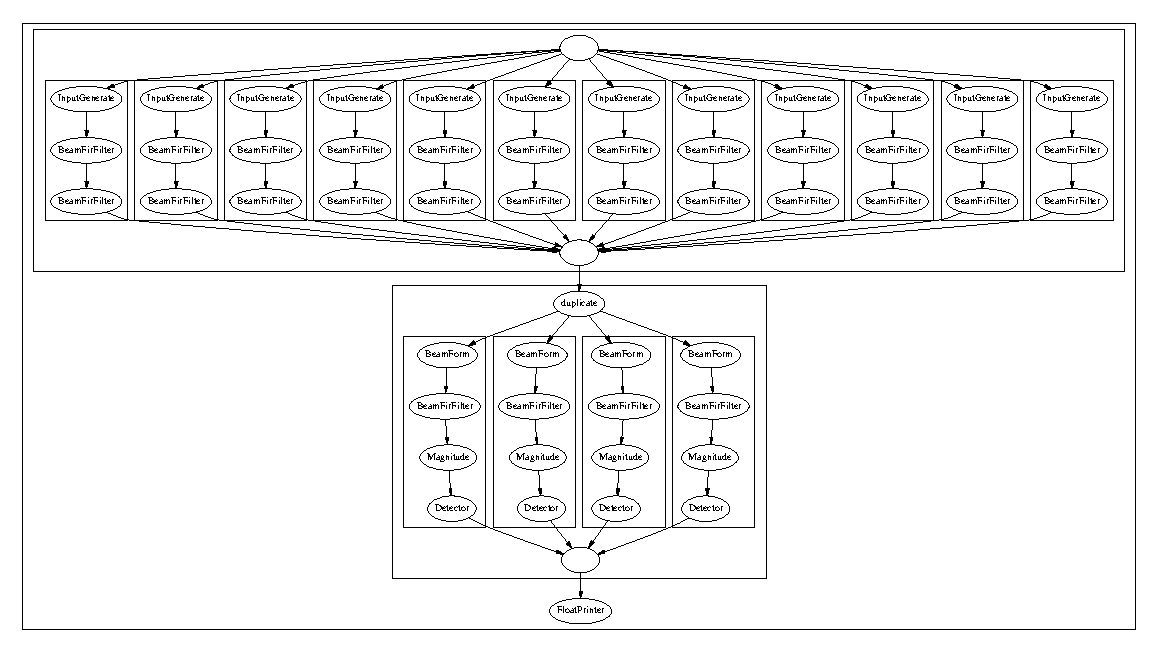
\includegraphics[width=5.0in]{figures/beamformer.eps}
%%   \caption{A DSP block diagram of the application Beamformer}
%%   \label{fig:block-diagram}
%% \end{figure}

%%     Blocks can be characterized in various ways. The simplest characterization
%% of blocks is a \textit{linear} block, defined as a module that
%% outputs a linear combination of its inputs plus a constant term. A
%% linear block can be represented by a matrix relating inputs to
%% outputs and a vector of constants. The next simplest
%% characterization of blocks is \textit{linear state space}. Such a
%% block uses a set of state variables. The output of this block is a
%% linear combination of its inputs and state variables. In addition,
%% the state variables are updated by a linear combination of
%% themselves and inputs.  A linear state space block can be
%% represented by four independent matrices.

%%     A linear state space characterization is more general than a
%% linear characterization - all linear blocks are also linear
%% state space blocks, but the converse is not true. The intuitive
%% reason for this fact is that a linear block is memoryless, meaning
%% the outputs only depend on current inputs. However, a linear
%% state space block has memory in the form of state variables, so
%% the outputs depend on current inputs and past inputs.

%%     We will perform analysis and optimization of DSP applications at
%% the linear state space level. We choose this representation
%% because it models a wide class of applications or parts of
%% applications, and it is simple to work with.

%%     Our work with state space representations will be done in the
%% context of StreamIt, a programming language designed for streaming
%% applications \cite{streamitcc}.  StreamIt allows users to create
%% their own blocks, but limits the way these blocks can be
%% connected. We perform the following steps on a StreamIt program:

%% \begin{enumerate}
%% \vspace{\itemshrink} \item Examine each block and determine whether or not it can be
%% characterized as linear state space. If it can, extract the
%% appropriate state space representation.

%% \vspace{\itemshrink} \item Combine connected blocks that each have a state space
%% representation, using an appropriate set of rules depending on the
%% type of connection.

%% \vspace{\itemshrink} \item Optimize representations through the use of state space
%% transformations.

%% \vspace{\itemshrink} \item Convert the state space representation(s) back to StreamIt
%% code.
%% \vspace{\itemshrink} \end{enumerate}

%% \mysubsection{Organization}

\begin{figure}[t]
\vspace{6pt}
{\small
\begin{verbatim}
   float->float filter MovingAverage(int N) {
     float[N] weights;  // a filter field

     // init function initializes the weights
     init {
       for (int i=0; i<N; i++)
         weights[i] = 1/N;
     }

     // work function declares push, pop, peek rates
     work push 1 pop 1 peek N {
       float result = 0;  // a local variable
       for (int i=0; i<N; i++) {
         result += weights[i] * peek(i);
       }
       push(result);
       pop();
     }
   } 
\end{verbatim}
\vspace{-12pt}
\caption{Example of a StreamIt filter.\protect\label{fig:filter-example}}}
\vspace{-6pt}
\end{figure}

\mysubsection{The StreamIt Language}
\label{sec:background}

StreamIt~\cite{streamitcc} is an architecture-independent language for
signal processing applications.  The model of computation in StreamIt
is Synchronous Dataflow~\cite{lee87static}, in which independent
filters communicate at fixed rates over FIFO channels.  StreamIt aims
to expose the abundant parallelism and regular communication patterns
in stream programs for the benefit of the compiler.  The optimizations
described in this paper would be infeasible in a general-purpose
language such as C.  As detailed elsewhere~\cite{streamitcc}, C
obscures the high-level structure of a streaming application due to
possible aliasing between autonomous filters, complex modulo
expressions on circular buffers, and interleaving of atomic execution
steps with global control flow.
%There is not enough information in C code to automatically perform the
%high-level transformations that experts use to achieve competitive
%performance.  
In addition, StreamIt offers improved programmer productivity over C
due to its parameterizable and composable stream constructs.

The basic programmable unit in StreamIt is a filter, which executes a
user-defined work function as its atomic execution step; for example,
see the {\tt MovingAverage} filter in Figure~\ref{fig:filter-example}.
Filters communicate with each other using FIFO channels.  On each
execution, a filter consumes ({\it pops}) a fixed number of items from
its input channel and produces ({\it pushes}) a fixed number of items
to its output channel.  A filter can also {\it peek} at a given index
on its input channel without consuming the item; this makes it simple
to write sliding-window applications such as the {\tt MovingAverage}.
The push, pop, and peek rates are declared on the same line as the
work function, thereby enabling the compiler to construct a static
schedule of filter firings~\cite{lee87static}.

Each filter has a distinct address space.  A filter can store two
types of variables: a {\it field} and a {\it local}.  Fields are
declared in the scope of the filter and are preserved across
executions, while locals are declared inside the work function and are
only live within a single execution.  There is also an init function,
run once at the beginning of the program, that can be used to
initialize fields.

StreamIt provides three hierarchical structures for composing filters
into larger stream graphs (see Figure~\ref{fig:structures}).  The {\it
pipeline} construct composes streams in sequence, with the output of
one connected to the input of the next.  The {\it splitjoin} construct
distributes data to a set of parallel streams, which are then joined
together in a roundrobin fashion.  The {\it feedback loop} provides a
mechanism for introducing cycles in the graph.  An example of a
pipeline appears in Figure~\ref{fig:iir-pipeline}.  It contains a
single Infinite Impulse Response (IIR) filter, which could be
implemented as shown at the top of Figure~\ref{fig:opt-seq}.

%%         A filter can store two types of variables - \textit{field} and
%% \textit{local}. Field variables are declared outside of the
%% specific functions (work, prework, init), and can be accessed from
%% anywhere within the filter. Local variables are declared within a
%% specific function, and only have scope within that function. For
%% example, a variable declared within the init function is local,
%% and could not be accessed within the work function. Therefore, the
%% init function is used to initialize field variables.

\mysubsection{State Space Example}
\begin{figure*}[t]
\begin{singlespace}

~~~~~
\begin{minipage}{0.46in}
{\centering
\psfig{figure=pipeline.eps,width=0.46in} \\
}
\end{minipage} 
~
\begin{minipage}{1.3in}
{\centering
\psfig{figure=splitjoin.eps,width=1.3in} \\
}
\end{minipage}
~
\begin{minipage}{1.02in}
{\centering
\psfig{figure=feedback.eps,width=1.02in} \\
}
\end{minipage}
~~~~~~~~~~~~
\begin{minipage}{3in}
\vspace{36pt}
\psfig{figure=iir-pipeline.eps, width=2.33in}
~~~~
\raisebox{12pt}{\psfig{figure=iir-pipeline2.eps, width=0.46in}}
\end{minipage}
\\ ~ \\ {\mbox{~~~}\protect\small \mbox{~}(a) A pipeline. ~~~~(b) A splitjoin. ~~~~~~~~(c) A feedbackloop.}

~\begin{minipage}{3.5in}
\caption{Stream structures supported by StreamIt.
\protect\label{fig:structures}}
\end{minipage}
~~~~~~
\begin{minipage}{3in}
\caption{Example pipeline with IIR filter.\protect\label{fig:iir-pipeline}}
\end{minipage}
\vspace{6pt}
\hrule
\vspace{6pt}

\hfill
\begin{minipage}{2.2in}
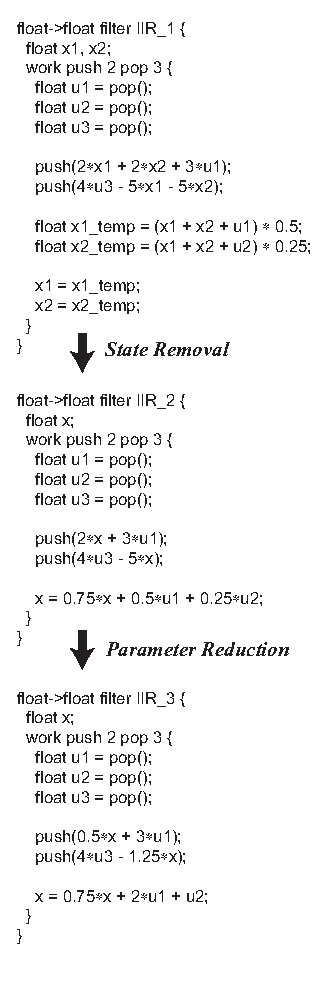
\epsfig{file=statespace-example.eps, width=2.05in}
\end{minipage}
~~~~
\raisebox{11pt}{
\begin{minipage}{3.5in}
\vspace{20pt}
Number of multiplications: 8 \\
Number of additions: 8 \\
State space representation:
\begin{eqnarray*}
\small
\vec{\dot{\mathbf{x}}} & = & \left [ \begin{array} {cc} 0.5 & 0.5 \\ 0.25
& 0.25 \end{array} \right ] \vec{\mathbf{x}} + \left [ \begin{array} {ccc} 0.5 & 0 & 0 \\
0 & 0.25 & 0 \end{array} \right ] \vec{\mathbf{u}} \\
\vec{\mathbf{y}} & = & \left [ \begin{array} {cc} 2 & 2 \\ -5 & -5
\end{array} \right ] \vec{\mathbf{x}} + \left [ \begin{array} {ccc} 3 & 0 & 0 \\ 0 & 0 & 4 \end{array} \right
 ] \vec{\mathbf{u}}
\end{eqnarray*}
\vspace{16pt} ~ \\
\hrule
\vspace{34pt} ~ \\
Number of multiplications: 7 \\
Number of additions: 4 \\
State space representation:
\begin{eqnarray*}
\small
\vec{\dot{\mathbf{x}}} & = & \left [ \begin{array} {cc} 0.75
\end{array} \right ] \vec{\mathbf{x}} + \left [ \begin{array} {ccc} 0.5 & 0.25 & 0 \end{array} \right ] \vec{\mathbf{u}} \\
\vec{\mathbf{y}} & = & \left [ \begin{array} {cc} 2 \\ -5
\end{array} \right ] \vec{\mathbf{x}} + \left [ \begin{array} {ccc} 3 & 0 & 0 \\ 0 & 0 & 4 \end{array} \right
 ] \vec{\mathbf{u}}
\end{eqnarray*}
\vspace{20pt} ~ \\
\hrule
\vspace{30pt} ~ \\
Number of multiplications: 5 \\
Number of additions: 4 \\
State space representation:
\begin{eqnarray*}
\small
\vec{\dot{\mathbf{x}}} & = & \left [ \begin{array} {cc} 0.75
\end{array} \right ] \vec{\mathbf{x}} + \left [ \begin{array} {ccc} 1 & 0.5 & 0 \end{array} \right ] \vec{\mathbf{u}} \\
\vec{\mathbf{y}} & = & \left [ \begin{array} {cc} 1 \\ -2.5
\end{array} \right ] \vec{\mathbf{x}} + \left [ \begin{array} {ccc} 3 & 0 & 0 \\ 0 & 0 & 4 \end{array} \right
 ] \vec{\mathbf{u}}
\end{eqnarray*}
\end{minipage}}
\end{singlespace}
\begin{center}
\vspace{-23pt}

\caption{Example optimization of an IIR filter using linear state
space analysis.  The top segment shows the original code.  The middle
segment depicts the action of state removal, in which the quantity
$x_1 + x_2$ is replaced by a single variable $x$.  The bottom segment
illustrates parameter reduction, in which the coefficients are
refactored so as to eliminate two multiplications (two coefficients
assume a value of 1).\protect\label{fig:opt-seq}}
\end{center}
\vspace{-12pt}
\end{figure*}


As described previously, a linear state space model describes a stream
in which both the outputs and the state values are updated as a linear
combination of the inputs and the previous states.  We use the
following notation to describe such systems:
\starteqnstar 
\vec{\dot{\mathbf{x}}} & = & \mathbf{A}\vec{\mathbf{x}} +
\mathbf{B}\vec{\mathbf{u}} \\
\vec{\mathbf{y}}
& = & \mathbf{C}\vec{\mathbf{x}} + \mathbf{D}\vec{\mathbf{u}}
\doneeqnstar
\noindent In these equations, the state vector is denoted by
$\vec{\mathbf{x}}$, the inputs by $\vec{\mathbf{u}}$, and the outputs
by $\vec{\mathbf{y}}$. $\vec{\dot{\mathbf{x}}}$ represents the new
\clearpage \noindent 
state vector, i.e., the state vector after it is updated.  The 
first equation is for the state updates, while the second equation is
for the outputs.  $\mathbf{A}$, $\mathbf{B}$, $\mathbf{C}$, and
$\mathbf{D}$ are matrices whose dimensions depend on the 
number of states, inputs, and outputs.

\looseness+1 Figure~\ref{fig:opt-seq} illustrates an optimization sequence for an
IIR filter.  Three versions of the filter are shown: original,
following state removal, and following parameter reduction.  In each
case, the state space representation for the filter is shown on the
right, along with the number of multiplications and additions needed
per execution of the work function.

\looseness+1 The state removal optimization identifies that the states
$x_1$ and $x_2$ are always used as part of the expression $x_1 + x_2$.
Thus, one of the states can be eliminated in favor of a single
variable, $x$, that tracks the value of the sum.  While relatively
simple in this example, such a transformation can be quite subtle when
applied to a large representation (e.g., the result of combining many
filters together.)  State removal can reduce storage requirements as
well as eliminate arithmetic operations (in this example, 1
multiplication and 4 additions).  As described in
Section~\ref{sec:state-removal}, state removal is formulated as a
general sequence of matrix operations.

The parameter reduction optimization refactors the coefficients that
operate on the state variables in order to reduce the number of
operations needed.  Following the transformation, $x$ assumes a value
that is twice as large as the original (at any given point of
execution).  However, this change does not affect the output of the
filter, as the coefficients in $\mathbf{A}$ are compensated
accordingly.  The transformation enables two coefficients in
$\mathbf{B}$ and $\mathbf{C}$ to change to a value of 1, thereby
eliminating two multiplication operations.  As described in
Section~\ref{sec:parameter-reduction}, this transformation is also
formulated as a general series of matrix operations.

\mysection{State Space Analysis}
\label{sec:statespace}

Our analysis operates on a symbolic representation of linear state
space filters.  We analyze the code of each StreamIt filter to
determine whether or not it is state space; if so we initialize a data
structure, fill it with the appropriate values through a process
called \emph{extraction}, and associate the structure with the filter.
We provide a set of rules to combine state space representations of
filters in hierarchical StreamIt blocks---pipelines, splitjoins, and
feedback loops. Such a process results in a single state space
representation for the entire block.  We also describe how to
\emph{expand} a representation so that it can be combined with blocks
of mis-matching dimensions.

\mysubsection{Representation}

Our first task is to create a data structure that fully captures the
state space representation of a StreamIt filter.  We save a filter's
number of states, push rate, and pop rate in variables termed $s$,
$u$, and $o$, respectively. Our data structure also contains the
matrices $\mathbf{A}$, $\mathbf{B}$, $\mathbf{C}$, and $\mathbf{D}$
with dimensions $s \times s$, $s
\times o$, $u \times s$, and $u \times o$, respectively. The
inputs to a filter are denoted by $\vec{\mathbf{u}}$ (length $o$), the
outputs by $\vec{\mathbf{y}}$ (length $u$), and the states by
$\vec{\mathbf{x}}$ (length $s$). Upon every execution of the filter,
we can update the state vector by the
formula $\vec{\dot{\mathbf{x}}} = \mathbf{A}\vec{\mathbf{x}} +
\mathbf{B}\vec{\mathbf{u}}$ and calculate the outputs by the formula $\vec{\mathbf{y}} =
\mathbf{C}\vec{\mathbf{x}} +
\mathbf{D}\vec{\mathbf{u}}$.  For convenience, we calculate the filter 
outputs before updating the
state vector. Since the states may have initial values other than
zero, we store these values as the vector
$\overrightarrow{\mathbf{initVec}}$ (length $s$).

Since we have not included a constant term in our model, we always set
one of the state variables to be the constant $1$. This variable is
not updated by any of the inputs or states (besides itself), and its
initial value is $1$, so it always remains that value. Any state or
output that depends on a constant term can now refer to a multiple of
the constant state variable instead.

As long as a filter's peek rate (denoted by $e$) equals its pop rate,
the data structure as currently described can fully represent the
filter. We must make additional modifications for a filter with a peek
rate greater than its pop rate. Note that such a filter still removes
$o$ items from its input tape upon every execution, but it accesses
$e-o$ additional items on its input tape. Therefore, our current data
structure would work as long as there is some way to access these
additional items.

We solve the problem of having a peek rate greater than a pop rate by
storing $e-o$ items from the input tape in the state vector
$\vec{\mathbf{x}}$.  Thus, when a filter executes, it can access all
$e$ items it needs: $o$ items from its input vector and $e-o$ items
from its state vector. These $e-o$ states must be updated by the
inputs and themselves---the specifics are covered in the next
section. We store the number of states used for inputs as the variable
$\mt{stored}$. This will be useful when combining representations.

When a filter is executed for the first time, it has access to the $o$
items in the input vector, but the $e-o$ states it needs have yet to
be copied from the input.  Therefore, we need to initialize the state
vector before iteratively computing the output and state update
equations.  We introduce a new matrix $\mathbf{B_{pre}}$ to perform
this initialization. Before the filter runs, it performs the state
update $\vec{\dot{\mathbf{x}}} =
\overrightarrow{\mathbf{initVec}} +
\mathbf{B_{pre}}\vec{\mathbf{u}}_\mathbf{pre}$. The initialization input
vector $\vec{\mathbf{u}}_\mathbf{pre}$ has length $o_{pre} =
e-o$. For now, $o_{pre}$ and $\mt{stored}$ have the same value, but
combining filters might result in $o_{pre}$ being greater than
$\mt{stored}$.

Putting these pieces together, a full representation consists of the
push and pop rates, the number of state variables, the number of
stored inputs, the four state matrices, an initial state vector, and
possibly an initialization state matrix and an initial pop rate. We
define a state space representation $\cal{R}$ as the tuple
$\langle$$u$, $o$, $s$, $\mt{stored}$, $\mathbf{A}$, $\mathbf{B}$,
$\mathbf{C}$, $\mathbf{D}$, $\overrightarrow{\mathbf{initVec}}$,
$\mathbf{B_{pre}}$, $o_{pre}$$\rangle$. When we introduce a
representation ${\cal R}_i$, each of its values in the ordered set
will be denoted with the index $i$ (for example $u_i$,
$\mathbf{A_i}$). For representations of filters that do not need the
initialization matrix, we write $\mathbf{B_{pre}} = \mt{null}$ and
$o_{pre} = 0$. In this case, the filter does not have any stored
inputs, so $\mt{stored} = 0$ as well.

Representations are initially created from StreamIt filters and
ultimately converted back to StreamIt filters. Between these steps,
however, representations of hierarchical StreamIt blocks can be
derived by combining the representations of their parts.  Thus, from
now on we will say that a representation refers to a block rather than
a filter. The exception is in the following section, where we discuss
how to create a representation from a StreamIt filter.
% Hence we explicitly refer to a filter rather than block
%representation in that section.

\mysubsection{Extraction}

We use a simple dataflow analysis to extract a state space
representation from the imperative code in a filter's work function.
While an alternate approach would be to allow the user to specify the
representation explicitly (as part of the program), StreamIt aims to
provide a unified development environment in which diverse filters are
implemented using a small set of primitives.  State space filters are
simple to implement using imperative StreamIt constructs, and in this
form they are immediately readable by programmers unfamiliar with the
state space formalism.

\looseness+1 Our dataflow analysis symbolically executes a single iteration of a
filter's work function, maintaining a vector pair representation for
each local variable and filter field that is encountered (together,
these are termed program variables). If the outputs and fields (i.e.,
states) all have vector pair representations, then the filter is
linear state space, and the vectors are used as rows of $\mathbf{A}$,
$\mathbf{B}$, $\mathbf{C}$, and $\mathbf{D}$.  Of course, many filters
do not fit the state space model; the optimizations developed in this
paper are selectively applied to the portions of the stream graph that
contain state space filters.
%See \cite{Lamb}
%for a treatment of the linear case.

\looseness+1 We attempt to find a vector pair ($\vec{\mathbf{v}}$,$\vec{\mathbf{w}}$) 
for each program variable $p$ such that $p = \vec{\mathbf{v}} \cdot
\vec{\mathbf{x}} + \vec{\mathbf{w}} \cdot \vec{\mathbf{u}}$, where  $\vec{\mathbf{x}}$ 
is the filter's state vector and $\vec{\mathbf{u}}$ is the filter's
input vector .  When $p$ is on the left hand side of an assignment
statement, terms from the right hand side are identified as states
(corresponding to entries of $\vec{\mathbf{x}}$) and inputs
(corresponding to entries of $\vec{\mathbf{u}}$).  The coefficients
from terms that match are used to fill the corresponding entries in
$\vec{\mathbf{v}}$ and $\vec{\mathbf{w}}$, as long as they are
constants. If any coefficient is not a constant, then $p$ is
non-linear.

The input vector $\vec{\mathbf{u}}$ is defined as $[\mt{peek}(e-o)
~\mt{peek}(e-o+1) ~... ~\mt{peek}(o-1)]$. The state vector
$\vec{\mathbf{x}}$ holds $e-o$ variables from the input tape
($\mt{peek}(0) ~... ~\mt{peek}(e-o-1)$), every filter field, and a
variable for the constant 1. We do not consider local variables for
the state vector, because their values are not saved across filter
executions.
%Therefore, their values should be resolved to
%constants at compile time. 
A filter field has the initial vector pair ($\left [ \begin{array}
{ccccc} 0 & ... & 1 & ... & 0 \end{array} \right ]$,
$\vec{\mathbf{0}}$), where the 1 corresponds to the field
itself.

If a vector pair is found for a given program variable $p$, then $p$
can be written as a linear combination of the inputs and state
variables, with the vector pair entries representing the weights.  The
final assignment to state variable $x_i$ by some program variable
$p_k$ indicates that the $i$th rows of $\mathbf{A}$ and $\mathbf{B}$
should be $\vec{\mathbf{v}}_\mathbf{k}$ and
$\vec{\mathbf{w}}_\mathbf{k}$, respectively. Similarly, if the $i$th
push statement uses program variable $p_k$, then the $i$th rows of
$\mathbf{C}$ and $\mathbf{D}$ should be $\vec{\mathbf{v}}_\mathbf{k}$
and $\vec{\mathbf{w}}_\mathbf{k}$, respectively.
% NOT TRUE!  Should be 1 for the constant itself
%For the constant state
%variable $1$, the corresponding rows of $\mathbf{A}$ and $\mathbf{B}$
%are all zeros.

We use the same procedure in the init function to find the initial
values for each filter field.  However, we do not need a vector
$\vec{\mathbf{w}}$ for the inputs, since there are no inputs to the
init function. The initial value for each stored input is zero, and
the initial value for the constant state is $1$.

Finally, consider the stored input states (call them
$\vec{\mathbf{x}}_\mathbf{s}$). They are updated by the inputs;
however, if $\mt{stored} > o$, then some of the input states must be
updated by other input states. In particular, the first $\mt{stored}-o$
input states are updated by the last $\mt{stored}-o$ input states, and the
remaining $o$ input states are updated by the $o$ inputs. The update
is described by the equation:
\begin{eqnarray}
\label{eq:one}
\vec{\dot{\mathbf{x}}}_\mathbf{s} = \left [
\begin{array} {cc} \mathbf{0} & \mathbf{I} \\ \mathbf{0} &
\mathbf{0} \end{array} \right ] \vec{\mathbf{x}}_\mathbf{s} + \left [
\begin{array} {c} \mathbf{0} \\ \mathbf{I} \end{array} \right ]
\vec{\mathbf{u}}
\end{eqnarray}

We also create an initialization matrix to put values from the input
tape into the input states:
\starteqnstar
\vec{\dot{\mathbf{x}}}_\mathbf{s} = \mathbf{0} +
\mathbf{I} \vec{\mathbf{u}}_\mathbf{pre}
\doneeqnstar

%Stored inputs are updated as shown on every execution step.
%Therefore, we use $\mathbf{A_s}$ and $\mathbf{B_s}$ to describe this
%update, where the values of these two matrices are given in
%Equation~\ref{eq:one}.

\newpage \mysubsubsection{Extraction Example}
\enlargethispage{-1\baselineskip}

Consider another IIR filter.  Unlike the example in
Section~\ref{sec:background}, this filter uses peeking to read
elements from the tape without consuming them.
\begin{singlespace}
\small
\begin{verbatim}
float->float filter IIR() {
    float curr;  // example of a filter field
    work push 1 pop 1 peek 3 {
      float temp; // example of a local variable
      temp = (peek(0) + peek(1) + peek(2))/6;
      curr = temp + curr/2;
      push(curr);
      pop();
    }
}
\end{verbatim}
\end{singlespace}
\vspace{-16pt}

\noindent The state vector is $\left [\hspace{-3.2pt}\begin{array} {c} \mt{peek}(0) \\ \mt{peek}(1) \\ curr \\ 1 \end{array} \hspace{-3.2pt}\right]$; the input vector is $\left [\hspace{-3.2pt}\begin{array} {c} \mt{peek}(2) \end{array} \hspace{-3.2pt}\right]$. The first program
variable encountered is $\mt{temp}$. It is given the vector pair
($\left [\begin{array} {cccc} 1/6 & 1/6 & 0 & 0 \end{array} \right ]$, $\left [ \begin{array} {c} 1/6 \end{array} \right ]$). The
variable $\mt{curr}$, as a state variable, has an initial vector pair:
($\left [\begin{array} {cccc} 0 & 0 & 1 & 0 \end{array} \right ]$, $\left [ \begin{array} {c} 0 \end{array} \right ]$). 
When $\mt{curr}$ is found in an assignment
statement, it is given a new vector pair, constructed as the vector
pair for $\mt{temp}$ plus $1/2$ times the old vector pair for $\mt{curr}$:
($\left [ \begin{array} {cccc} 1/6 & 1/6 & 1/2 & 0 \end{array}
\right ]$, $\left [ \begin{array} {c} 1/6 \end{array} \right ]$). 
The output is $\mt{curr}$, so it is given the same vector
pair. The final pair for $\mt{curr}$ represents its state update. The
stored inputs $\mt{peek}(0)$ and $\mt{peek}(1)$ are updated as in
Equation~\ref{eq:one}, and the constant $1$ updated to itself. Therefore,
we have:

\begin{minipage}{1.6in}
\starteqnstar
\mathbf{A} = \left [ \begin{array} {cccc} 0 & 1 & 0 & 0 \\ 0 &
0 & 0 & 0 \\ 1/6 & 1/6 & 1/2 & 0 \\ 0 & 0 & 0 & 1 \end{array}
\right ]
\doneeqnstar
\end{minipage}
\begin{minipage}{1.4in}
\starteqnstar
\mathbf{B} = \left [ \begin{array} {c} 0 \\ 1 \\ 1/6 \\ 0
\end{array} \right ]
\doneeqnstar
\end{minipage}

\begin{minipage}{1.57in}
\starteqnstar
\mathbf{C} = \left [ \begin{array} {cccc} 1/6 & 1/6 & 1/2 & 0
\end{array} \right ]
\doneeqnstar
\end{minipage}
\begin{minipage}{1.4in}
\starteqnstar
\mathbf{D} = \left [ \begin{array} {c} 1/6 \end{array} \right ]
\doneeqnstar
\end{minipage}

\begin{minipage}{1in}
\starteqnstar
\overrightarrow{\mathbf{initVec}} = \left [ \begin{array} {c}
0 \\ 0 \\ 0 \\ 1 \end{array} \right ]
\doneeqnstar
\end{minipage}
\hspace{0.76in}
\begin{minipage}{1in}
\starteqnstar
\mathbf{B_{pre}} = \left [ \begin{array} {cc} 1 & 0 \\ 0 & 1
\\ 0 & 0 \\ 0 & 0 \end{array} \right ]
\doneeqnstar
\end{minipage} ~\\

The pop and push rates are both 1, and there are four states, so $o =
1$, $u = 1$, and $s = 4$.  There are two stored input states, so
$o_{pre} = 2$ and $\mt{stored} = 2$.

\mysubsection{Combination}

If all blocks within a given pipeline, splitjoin, or feedback loop
have state space representations, they can be combined into a single
representation using the rules developed in this section.  There are
two benefits to combining blocks.  First, combination can eliminate
redundant computations across blocks.  Second, combination exposes
optimization opportunities, as intra-block optimizations (described in
Section~\ref{sec:optimization}) can effectively be applied across
blocks by combining the blocks first.

\mysubsubsection{Pipeline}
\label{sec:pipeline}

Consider two blocks connected in a pipeline with representations
${\cal R}_1$ and ${\cal R}_2$.  We will derive the combined
representation of the two blocks, denoted by ${\cal R}$.  Suppose the
output rate of ${\cal R}_1$ equals the input rate of ${\cal R}_2$
($u_1 = o_2$). If this is not the case, we must expand one or both
blocks to have their input/output rates match ($u_1' =
o_{2}' = lcm(u_1,o_2)$). Block expansion is covered in
Section~\ref{sec:expansion}. Since the output of ${\cal R}_1$ (i.e.,
$\vec{\mathbf{y}}_\mathbf{1}$) is equivalent to the input of ${\cal
R}_2$ (i.e., $\vec{\mathbf{u}}_\mathbf{2}$), we can write:
\starteqnstar
\vec{\dot{\mathbf{x}}}_{{{\mathbf 1}}} & = & \mathbf{A_1}\vec{\mathbf{x}}_{{\mathbf 1}} + \mathbf{B_1}\vec{\mathbf{u}}_{{\mathbf 1}} \\
\vec{\dot{\mathbf{x}}}_{{{\mathbf 2}}} & = & \mathbf{A_2}\vec{\mathbf{x}}_{{\mathbf 2}} + \mathbf{B_2}\vec{\mathbf{y_1}} \\[1.5Ex]
\vec{\mathbf{y}}_{{\mathbf 1}} & = & \mathbf{C_1}\vec{\mathbf{x}}_{{\mathbf 1}} + \mathbf{D_1}\vec{\mathbf{u}}_{{\mathbf 1}} \\
\vec{\mathbf{y}}_{{\mathbf 2}} & = & \mathbf{C_2}\vec{\mathbf{x}}_{{\mathbf 2}} +
\mathbf{D_2}\vec{\mathbf{y}}_{{\mathbf 1}}
\doneeqnstar
Substituting for $\vec{\mathbf{y}}_{{\mathbf 1}}$ yields:
\starteqnstar
\vec{\dot{\mathbf{x}}}_{{{\mathbf 2}}} & = & \mathbf{A_2}\vec{\mathbf{x}}_{{\mathbf 2}} + \mathbf{B_2}(\mathbf{C_1}\vec{\mathbf{x}}_{{\mathbf 1}} + \mathbf{D_1}\vec{\mathbf{u}}_{{\mathbf 1}} \\
\vec{\mathbf{y}}_{{\mathbf 2}} & = & \mathbf{C_2}\vec{\mathbf{x}}_{{\mathbf 2}} +
\mathbf{D_2}(\mathbf{C_1}\vec{\mathbf{x}}_{{\mathbf 1}} +
\mathbf{D_1}\vec{\mathbf{u}}_{{\mathbf 1}})
\doneeqnstar
Which simplifies to:
\starteqnstar
\vec{\dot{\mathbf{x}}}_{{{\mathbf 2}}} & = & \mathbf{A_2}\vec{\mathbf{x}}_{{\mathbf 2}} + \mathbf{B_2}\mathbf{C_1}\vec{\mathbf{x}}_{{\mathbf 1}} + \mathbf{B_2}\mathbf{D_1}\vec{\mathbf{u}}_{{\mathbf 1}} \\
\vec{\mathbf{y}}_{{\mathbf 2}} & = & \mathbf{C_2}\vec{\mathbf{x}}_{{\mathbf 2}} +
\mathbf{D_2}\mathbf{C_1}\vec{\mathbf{x}}_{{\mathbf 1}} +
\mathbf{D_2}\mathbf{D_1}\vec{\mathbf{u}}_{{\mathbf 1}}
\doneeqnstar

Let $\vec{\mathbf{x}} = \left [ \begin{array} {c} \vec{\mathbf{x}}_{{\mathbf 1}} \\
\vec{\mathbf{x}}_{{\mathbf 2}} \end{array} \right ]$, $\vec{\mathbf{u}} =
\vec{\mathbf{u}}_{{\mathbf 1}}$ (the input to the entire pipeline), and
$\vec{\mathbf{y}} = \vec{\mathbf{y}}_{{\mathbf 2}}$ (the output of the entire
pipeline). The equations relating $\vec{\mathbf{x}}$,
$\vec{\mathbf{u}}$, and $\vec{\mathbf{y}}$ are:
\starteqnstar
\vec{\dot{\mathbf{x}}} & = & \mathbf{A}\vec{\mathbf{x}} + \mathbf{B}\vec{\mathbf{u}} \\
\vec{\mathbf{y}} & = & \mathbf{C}\vec{\mathbf{x}} + \mathbf{D}\vec{\mathbf{u}}
\doneeqnstar ~ \\ \vspace{-36pt} ~ \\
\starteqnstar
\mathbf{A} = \left [ \begin{array} {cc} \mathbf{A_1} &
\mathbf{0} \\ \mathbf{B_2}\mathbf{C_1} & \mathbf{A_2} \end{array} \right ] &~&
\mathbf{B} = \left [ \begin{array} {c} \mathbf{B_1} \\ \mathbf{B_2}\mathbf{D_1} \end{array} \right ] \\ ~&~&~ \\
\mathbf{C} = \left [ \begin{array} {cc} \mathbf{D_2}\mathbf{C_1} & \mathbf{C_2} \end{array} \right ] &~&
\mathbf{D} = \mathbf{D_2}\mathbf{D_1}
\doneeqnstar

The input to the pipeline is identical to the input to ${\cal R}_1$,
and the output of the pipeline is identical to the output of
${\cal R}_2$. Furthermore, the states of the pipeline are the states
of the first block appended to the states of the second
block. Thus, $u = u_2$, $o = o_1$, $s = s_1 + s_2$, and 
$\overrightarrow{\mathbf{initVec}} = \left [ \begin{array} {c}
\overrightarrow{\mathbf{initVec}_\mathbf{1}} \\ \overrightarrow{\mathbf{initVec}_\mathbf{2}}
\end{array} \right ]$.

If neither block has an initialization matrix, then the entire
pipeline does not need an initialization matrix, so $\mathbf{B_{pre}}
= \mt{null}$, $o_{pre} = 0$, and $\mt{stored} = 0$. If only the first block
has an initialization matrix, then we initialize the states in the
pipeline corresponding to the first block while keeping the states
corresponding to the second block unchanged:
\starteqnstar
~~~~ \mathbf{B_{pre}} = \left [ \begin{array} {c} \mathbf{B_{pre1}} \\ \mathbf{0} \end{array} \right ]
~~~~ o_{pre} = o_{pre1} 
~~~~ stored = stored_1
\doneeqnstar

If the second block has an initialization matrix, the first block must
run enough times to provide the necessary inputs to initialize the
second block. However, this might result in the first block providing
extra initial inputs to the second block. In that case, we must change
the representation of the second block to increase its number of
stored inputs.  A full description of this case appears
in~\cite[pp. 46-49]{Agrawal04}.

If there are more than two blocks in a pipeline, they can be collapsed
in the following manner: first combine the first two blocks to get one
block representation, then combine this representation with the third
block, and so on.

\mysubsubsection{Splitjoin and Feedback Loop}

The combination rules for splitjoins and feedback loops are somewhat
involved, and we omit them due to space considerations.  An important
benefit of a linear state space representation over a linear
representation is that feedback loops can be collapsed; the items on
the feedback path become states in the combined block.  A thorough
treatment of these cases appears in~\cite[pp. 36-43]{Agrawal04}.

\mysubsection{Expansion}
\label{sec:expansion}

Sometimes it is necessary to simulate multiple executions of a block
in order to combine it properly with other blocks.  For example,
suppose block $B_1$ outputs two items and block $B_2$ inputs five
items. In order to combine these blocks in a pipeline, $B_1$ must run
five times (in order to output ten items) and $B_2$ must run two times
(in order to input ten items). Therefore, a method is needed to expand
a representation so that it models a block running multiple times,
rather than once.

Consider the state space equation pair, where $\vec{\mathbf{u}}_{{\mathbf 1}}$ and
$\vec{\mathbf{y}}_{{{\mathbf 1}}}$ are the first set of inputs and outputs, and
$\vec{\mathbf{x}}$ is the original state vector:
\starteqnstar
\vec{\dot{\mathbf{x}}} & = & \mathbf{A}\vec{\mathbf{x}} + \mathbf{B}\vec{\mathbf{u}}_{{\mathbf 1}} \\
\vec{\mathbf{y}}}_{{{\mathbf 1}} & = & \mathbf{C}\vec{\mathbf{x}} +
\mathbf{D}\vec{\mathbf{u}}_{{\mathbf 1}}
\doneeqnstar

If we run the block again, the equation pair in terms of the
original state vector $\vec{\mathbf{x}}$ and the next set of
inputs and outputs ($\vec{\mathbf{u}}_{{\mathbf 2}}$ and $\vec{\mathbf{y}}_{{\mathbf 2}}$)
is:
\starteqnstar
\vec{\dot{\mathbf{x}}} & = & \mathbf{A}(\mathbf{A}\vec{\mathbf{x}}
+
\mathbf{B}\vec{\mathbf{u}}_{{\mathbf 1}}) + \mathbf{B}\vec{\mathbf{u}}_{{\mathbf 2}} \\
\vec{\mathbf{y}}}_{{{\mathbf 2}} & = & \mathbf{C}(\mathbf{A}\vec{\mathbf{x}} +
\mathbf{B}\vec{\mathbf{u}}_{{\mathbf 1}}) + \mathbf{D}\vec{\mathbf{u}}_{{\mathbf 2}}
\doneeqnstar
\noindent Simplifying yields:
\starteqnstar
\vec{\dot{\mathbf{x}}} & = & \mathbf{A}^2\vec{\mathbf{x}} +
\mathbf{AB}\vec{\mathbf{u}}_{{\mathbf 1}} + \mathbf{B}\vec{\mathbf{u}}_{{\mathbf 2}} \\
\vec{\mathbf{y}}}_{{{\mathbf 2}} & = & \mathbf{CA}\vec{\mathbf{x}} +
\mathbf{CB}\vec{\mathbf{u}}_{{\mathbf 1}} + \mathbf{D}\vec{\mathbf{u}}_{{\mathbf 2}}
\doneeqnstar

Let $\vec{\mathbf{u}}$ denote the combined input vector ($\vec{\mathbf{u}}
= \left [ \begin{array} {c} \vec{\mathbf{u}}_{{\mathbf 1}}
\\ \vec{\mathbf{u}}_{{\mathbf 2}} \end{array} \right ]$) and $\vec{\mathbf{y}}$ denote the 
combined output vector ($\vec{\mathbf{y}} = \left [ \begin{array} {c}
\vec{\mathbf{y}}_{{\mathbf 1}}
\\ \vec{\mathbf{y}}_{{\mathbf 2}} \end{array} \right ]$). The representation in terms of these two
vectors is:
\starteqnstar
\vec{\dot{\mathbf{x}}} & = & \mathbf{A_2}\vec{\mathbf{x}} + \mathbf{B_2}\vec{\mathbf{u}} \\
\vec{\mathbf{y}} & = & \mathbf{C_2}\vec{\mathbf{x}} + \mathbf{D_2}\vec{\mathbf{u}}
\doneeqnstar ~ \\ \vspace{-36pt} ~ \\
\starteqnstar
\mathbf{A_2} = \mathbf{A}^2 ~~~~~
\mathbf{B_2} = \left [ \begin{array} {cc} \mathbf{AB} & \mathbf{B} \end{array} \right ]  \\
\mathbf{C_2} = \left [ \begin{array} {c} \mathbf{C} \\
\mathbf{CA} \end{array} \right ] ~~~~~
\mathbf{D_2} = \left [ \begin{array} {cc} \mathbf{D} & \mathbf{0} \\
\mathbf{CB} & \mathbf{D} \end{array} \right ]
\doneeqnstar
This new representation corresponds to a block that, upon every
execution, runs the old block twice.  By induction, a general formula
for running a block $n$ times is:
\starteqnstar
\mathbf{A_n} = \mathbf{A}^n ~~~~~
\mathbf{B_n} = \left [ \begin{array} {ccccc} \mathbf{A}^{n-1}
\mathbf{B} & \mathbf{A}^{n-2} \mathbf{B} & ...  & \mathbf{AB} &
\mathbf{B} \end{array} \right ] \\
\mathbf{C_n} = \left [ \begin{array} {c} \mathbf{C} \\
\mathbf{CA} \\
... \\
\mathbf{CA^{n-2}} \\
\mathbf{CA^{n-1}} \end{array} \right ]~~~~~~~~~~~~~~~~~~~~~~~~~~~~~~~~~~~~~~~~~~~~~~~~~~~ \\
\mathbf{D_n} = \left [ \begin{array} {ccccccc}
\mathbf{D} & \mathbf{0} & \mathbf{0} & ... & \mathbf{0} & \mathbf{0} \\
\mathbf{CB} & \mathbf{D} & \mathbf{0} & ... & \mathbf{0} & \mathbf{0} \\
\mathbf{CAB} & \mathbf{CB} & \mathbf{D} & ... & \mathbf{0} & \mathbf{0} \\
... & ... & ... & ... & ... & ... \\
\mathbf{CA}^{n-3} \mathbf{B} & \mathbf{CA}^{n-4} \mathbf{B} &
\mathbf{CA}^{n-5} \mathbf{B} & ... & \mathbf{D} & \mathbf{0} \\
\mathbf{CA}^{n-2} \mathbf{B} & \mathbf{CA}^{n-3} \mathbf{B} &
\mathbf{CA}^{n-4} \mathbf{B} & ... & \mathbf{CB} &
\mathbf{D} \end{array} \right ]
%% following version is same but with one extra column and row
%% \mathbf{D_n} = \left [ \begin{array} {ccccccc}
%% \mathbf{D} & \mathbf{0} & \mathbf{0} & ... & \mathbf{0} & \mathbf{0} & \mathbf{0} \\
%% \mathbf{CB} & \mathbf{D} & \mathbf{0} & ... & \mathbf{0} & \mathbf{0} & \mathbf{0} \\
%% \mathbf{CAB} & \mathbf{CB} & \mathbf{D} & ... & \mathbf{0} & \mathbf{0} & \mathbf{0} \\
%% ... & ... & ... & ... & ... & ... & ... \\
%% \mathbf{CA}^{n-4} \mathbf{B} & \mathbf{CA}^{n-5} \mathbf{B} &
%% \mathbf{CA}^{n-6} \mathbf{B} & ... & \mathbf{D} & \mathbf{0} & \mathbf{0} \\
%% \mathbf{CA}^{n-3} \mathbf{B} & \mathbf{CA}^{n-4} \mathbf{B} &
%% \mathbf{CA}^{n-5} \mathbf{B} & ... & \mathbf{CB} & \mathbf{D} & \mathbf{0} \\
%% \mathbf{CA}^{n-2} \mathbf{B} & \mathbf{CA}^{n-3} \mathbf{B} &
%% \mathbf{CA}^{n-4} \mathbf{B} & ... & \mathbf{CAB} & \mathbf{CB} &
%% \mathbf{D} \end{array} \right ]
\doneeqnstar

Since initializations are not affected,
$\overrightarrow{\mathbf{initVec}}$, $\mathbf{B}_\mathbf{pre}$,
$\mt{stored}$, and $o_{pre}$ remain unchanged from the initial
representation. Since the number of states is not changed, $s$ remains
the same. The new representation runs the old representation $n$
times, so $u_{new} = n * u_{old}$ and $o_{new} = n * o_{old}$.

As mentioned in Section~\ref{sec:pipeline}, it is sometimes necessary
to simulate the initialization stage of a block (in addition to
simulating $n$ executions) for the purpose of initializing a full
pipeline.  In this case, the equations are very similar to above, but
also include terms for $\mathbf{B_{pre}}$.  Full details appear
in~\cite[pp. 45-46]{Agrawal04}.

\mysection{Optimizations}
\label{sec:optimization}

We consider two types of optimizations.  The first is to remove
redundant state variables from the linear state space representation.
This reduces the memory allocation for a program as well as the number
of loads and stores, which are typically slow and power-hungry
operations. It also eliminates computations that involve the removed
states.  The second optimization is to reduce the parametrization of a
state space representation by refactoring the matrices to contain more
zero and one entries.  This directly eliminates computations, as the
compiler statically evaluates $0 \cdot x = 0$ and $1 \cdot x = x$
rather than performing the multiplications at runtime.  Both the state
removal optimization and parameter reduction optimization are
formulated as a series of general transformations on the underlying
state space representation.

\mysubsection{State Space Transformations}

For any state space equation pair, there are an infinite number of
transformations to an equivalent state space system.  These
transformations involve a change of basis of the state vector
$\vec{\mathbf{x}}$ to $\mathbf{T} \vec{\mathbf{x}}$, where
$\mathbf{T}$ is an invertible matrix. Consider the state update
equation $\vec{\dot{\mathbf{x}}} = \mathbf{A} \vec{\mathbf{x}} +
\mathbf{B} \vec{\mathbf{u}}$. Multiplying the entire equation by
$\mathbf{T}$ yields:
\starteqnstar
\mathbf{T} \vec{\dot{\mathbf{x}}} = \mathbf{TA} \vec{\mathbf{x}} +
\mathbf{TB} \vec{\mathbf{u}}
\doneeqnstar
Since $\mathbf{T}^{-1} \mathbf{T} = \mathbf{I}$, we can write:
\starteqnstar
\mathbf{T} \vec{\dot{\mathbf{x}}} & = & \mathbf{TA}
(\mathbf{T}^{-1} \mathbf{T}) \vec{\mathbf{x}} + \mathbf{TB}
\vec{\mathbf{u}} ~~=~~ \mathbf{TA}
\mathbf{T}^{-1} (\mathbf{T} \vec{\mathbf{x}}) + \mathbf{TB} \vec{\mathbf{u}} \\
\vec{\mathbf{y}} & = & \mathbf{C} (\mathbf{T}^{-1} \mathbf{T})
\vec{\mathbf{x}} + \mathbf{D} \vec{\mathbf{u}} ~~~~~\hspace{1.1pt}~=~~ \mathbf{C}
\mathbf{T}^{-1} (\mathbf{T} \vec{\mathbf{x}}) + \mathbf{D}
\vec{\mathbf{u}}
\doneeqnstar
where we have introduced the output equation as well. Let
$\vec{\mathbf{z}} = \mathbf{T} \vec{\mathbf{x}}$.
$\vec{\mathbf{z}}$ is a new state vector related to the old state
vector $\vec{\mathbf{x}}$ by the change of basis $\mathbf{T}$.
Substituting into the above equations yields:
\starteqnstar
\vec{\dot{\mathbf{z}}} & = & \mathbf{TA} \mathbf{T}^{-1} \vec{\mathbf{z}} + \mathbf{TB} \vec{\mathbf{u}} \\
\vec{\mathbf{y}} & = & \mathbf{C} \mathbf{T}^{-1}\vec{\mathbf{z}}
+ \mathbf{D}\vec{\mathbf{u}}
\doneeqnstar

This is precisely the original state space equation pair,
with $\mathbf{A}$, $\mathbf{B}$, and $\mathbf{C}$ transformed to
$\mathbf{T} \mathbf{A} \mathbf{T}^{-1}$, $\mathbf{T} \mathbf{B}$,
and $\mathbf{C} \mathbf{T}^{-1}$, respectively.

For a StreamIt state space representation $\cal{R}$, we must determine
how the other values change.  Since the old state vector
$\vec{\mathbf{x}}$ is multiplied by $\mathbf{T}$, the old initial
state vector is multiplied by $\mathbf{T}$.  The initialization update
equation is analogous to the standard update equation, so
$\mathbf{B_{pre}}$ is transformed to $\mathbf{T} \mathbf{B_{pre}}$.  The
number of states, inputs, and outputs is the same, so $s$, $o$, and
$u$ are unchanged.

\mysubsection{State Removal}
\label{sec:state-removal}

There are two types of states that can be removed from a state space
system without changing its behavior: unreachable and unobservable
states.  Informally, unreachable states are unaffected by inputs and
unobservable states have no effect on outputs.  If there are two
redundant states in a filter, then both may reachable and observable
as the program is written.  However, following a series of
transformations, one of the redundant states can be converted to an
unreachable or unobservable state, allowing it to be removed.

More formally, the $i$th state is reachable if and only if at least
one of the following is true:
\begin{enumerate}
\item \parbox[t]{2.8in}{The state is initialized to a non-zero value.
That is, the $i$th entry of $\overrightarrow{\mathbf{initVec}}$ is
non-zero or $\exists j~\mbox{s.t.}~\mathbf{B_{pre}}[i,j] \ne 0$.}

\item \parbox[t]{2.8in}{The state directly depends on an input.  That
is, $\exists j~\mbox{s.t.}~\mathbf{B}[i,j] \ne 0$.}

\item \parbox[t]{2.8in}{The state directly depends on another
reachable state.  That is, $\exists j \ne
i~\mbox{s.t.}~\mathbf{A}[i,j] \ne 0$ and $j$ is a reachable state.}
\end{enumerate}
All states in the system are either reachable or unreachable.
Unreachable states always have a value of zero, as they are
initialized to zero and are never updated by a non-zero value (i.e.,
by a reachable state or an input).  Therefore, unreachable states can
be removed from the state space representation, since they have no
effect on any other states or output values.

The $i$th state is observable if and only if at least one of the
following is true:
\begin{enumerate}
\item \parbox[t]{2.8in}{An output directly depends on the state.  That
is, $\exists j~\mbox{s.t.}~\mathbf{C}[j,i] \ne 0$.}

\item \parbox[t]{2.8in}{Another observable state directly depends on
the state.  That is, $\exists j \ne i~\mbox{s.t.}~\mathbf{A}[j,i] \ne
0$ and $j$ is an observable state.}
\end{enumerate}
All states in the system are either observable or unobservable.  The
unobservable states are not used to update the observable states and
are not used to determine the outputs.  Therefore, all unobservable
states can be removed from a representation (regardless of their
initial values).

There is a simple algorithm to refactor the states of a system and
expose the unreachable and unobservable states~\cite{Mayne}.  For
unreachable states, the algorithm assumes that there is no
initialization stage, i.e., that $\overrightarrow{\mathbf{initVec}}$
and $\mathbf{B_{pre}}$ are zero.  We first describe the basic
algorithm and then extend it to handle the initialization stage.

To detect unreachable states, the algorithm performs row
operations\footnote{\smaller Performing a row operation operation on a
matrix is equivalent to left-multiplying it by some invertible matrix,
while performing a column operation is equivalent to right-multiplying
by some invertible matrix.} on the augmented matrix $\left [
\begin{array} {cc} \mathbf{A} & \mathbf{B} \end{array} \right ]$.  To 
maintain the proper input/output relationship of the system,
corresponding inverse column operations are performed on $\mathbf{A}$
and $\mathbf{C}$.  The row operations achieve a special type of
row-echelon form.  In this form, the last non-zero entry in each row
is a 1 (called the ending 1) and the ending 1 in a given row is to the
left of the ending 1 in lower rows.  Once the augmented matrix is in
the desired form, row $i$ represents an unreachable state if there are
no non-zero entries past the $i$th column.  This naturally expresses
the constraint that the $i$th state does not depend on any input
(columns of $\mathbf{B}$) or on any possibly reachable state (later
columns of $\mathbf{A}$).  In the absence of an initialization stage,
all unreachable states identified in this way can be removed from the
system.

For unobservable states, the same procedure is applied to the
augmented matrix $\left [\begin{array} {cc} \mathbf{A}^T &
\mathbf{C}^T \end{array} \right ]$.  In the echelon form, row $i$
represents an unobservable state if there are no non-zero entries past
the $i$th column.  Intuitively, the rows of the transposed matrices
represent how a given state is used, rather than how it is calculated.
The identified states are unobservable because they are used neither
in the calculation of an output (columns of $\mathbf{C}^T$) nor in
possibly observable states (later columns of $\mathbf{A}^T$).  All of
these unobservable states can be safely removed from the system (even
if they are assigned an initial value).

\looseness+1 To handle the initialization stage for unreachable
states, a minor extension is needed.  If a state is assigned a
non-zero value during initialization, either as a constant (a non-zero
entry in $\overrightarrow{\mathbf{initVec}}$) or from the input (a
non-zero entry in $\mathbf{B_{pre}}$), the state must be considered
reachable.  Further, any dependent states must also be considered
reachable.  This classification can easily be performed as a
post-processing step on the set of candidate unreachable states
identified by the algorithm above.  If any candidate is initialized to
a non-zero value or directly depends (via the $\mathbf{A}$ matrix) on
a state outside the set, then the candidate is removed from the set.
When no further candidate can be removed from the set, the set
contains nothing but genuine unreachable states.

%% The general algorithm for identifying unreachable states works as
%% follows.  First, it uses the previous algorithm~\cite{Mayne} to
%% identify {\it candidate} unreachable states.  Suppose that there are
%% $k$ candidates.  The candidate states are moved to the top of the
%% state vector via a series of row operations.  Following this
%% reordering, the sub-matrix $\mathbf{A}[1:k;1:k]$ represents the
%% dependences between candidate unreachable states.  As detailed below,
%% this sub-matrix is converted to an upper-triangular form (i.e., all
%% entries below the diagonal are zero) while maintaining the
%% input/output relationship of the system.  Finally, the candidate
%% states are considered in reverse order (from $k$ to $1$).  The $i$th
%% state is declared reachable if at least one of the following is true:
%% \begin{itemize}
%% \item The $i$th state is initialized to a non-zero value.

%% \item The $i$th state directly depends on another reachable state.
%% \end{itemize}

%%%%%%%%%%%%%%%%%%%%%%%%%%%%%%%%%%%%%%%%%%%%%%%%%%%%%%%%%

\mysubsubsection{Expanding the Scope}

So far we have considered optimizations that affect $\mathbf{A}$,
$\mathbf{B}$, and $\mathbf{C}$. Since the optimizations are entirely
the result of state transformations, they do not affect $\mathbf{D}$,
which is independent of the choice of state space basis.  However, if
all of the inputs are stored as states, then all of the entries of
$\mathbf{D}$ are moved into $\mathbf{A}$ and can then be changed by
state optimizations.

We have already discussed how to store inputs as states. When every
input is stored as a state, the new state-equation pair is:
\vspace{2pt}
\starteqnstar
\left [ \begin{array} {c} \vec{\dot{\mathbf{x}}} \\
\vec{\dot{\mathbf{x_{in}}}} \end{array} \right ] & = & \left [
\begin{array} {cc} \mathbf{A} & \mathbf{B} \\ \mathbf{0} &
\mathbf{0} \end{array} \right ] \left [ \begin{array} {c}
\vec{\mathbf{x}} \\ \vec{\mathbf{x}}_{{\mathbf{in}}} \end{array} \right ]
+ \left [ \begin{array} {c} \mathbf{0} \\ \mathbf{I} \end{array}
\right ] \vec{\mathbf{u}} \vspace{1pt} \\
\vec{\mathbf{y}} & = & \left [ \begin{array} {cc} \mathbf{C} &
\mathbf{D} \end{array} \right ] \left [ \begin{array} {c}
\vec{\mathbf{x}} \\ \vec{\mathbf{x}}_{{\mathbf{in}}} \end{array} \right ]
+ \mathbf{0} \vec{\mathbf{u}}
\doneeqnstar
\vspace{2pt}
These states should be added before state removal is performed. It may
seem counter-intuitive that we first add states, then seek to remove
them. However, the added states represent computations involving
$\mathbf{D}$ which were not considered before. Removing some of these
states can result in reducing computations involving $\mathbf{D}$.

\mysubsection{Parameter Reduction}
\label{sec:parameter-reduction}

After removing as many states as possible, additional computations can
be eliminated by transforming the state space system to one with fewer
non-zero, non-one entries (termed parameters). If $\mathbf{A}$,
$\mathbf{B}$, and $\mathbf{C}$ are completely filled, there are
$s*(s+o+u)$ parameters. Ackermann and Bucy \cite{Ackermann/Bucy} show
a general form in which $\mathbf{A}$ and $\mathbf{C}$ have at most
$s*(o+u)$ parameters ($\mathbf{B}$ may contain any number of
parameters), assuming there are no unobservable or unreachable
states. They derive this form using system impulse responses. We
achieve the same form using row operations on the augmented matrix
$\left [ \begin{array} {cc} \mathbf{A}^T & \mathbf{C}^T \end{array} \right ]$. 
The desired form is:

\newpage
~ \\ \vspace{-24pt}
\starteqnstar
\mathbf{A}^T &=& \left [ \begin{array} {ccccc} \mathbf{L_1} &
\mathbf{A_{12}} & \mathbf{A_{13}} & ... & \mathbf{A_{1u}} \\
\mathbf{0} & \mathbf{L_2} & \mathbf{A_{23}} & ... &
\mathbf{A_{2u}} \\ \mathbf{0} & \mathbf{0} & \mathbf{L_3} & ... &
\mathbf{A_{3u}} \\ ... & ... & ... & ... & ... \\ \mathbf{0} &
\mathbf{0} & \mathbf{0} & ... & \mathbf{L_u} \end{array} \right ] \\ ~ \\
\mathbf{C}^T &=& \left [ \begin{array} {ccccc} 1 & 0 & 0 & ... &
0 \\ 0 & 0 & 0 & ... & 0 \\ ... & ... & ... & ... & ... \\ 0 & 1 &
0 & ... & 0 \\ 0 & 0 & 0 & 0 & 0 \\ ... & ... & ... & ... & ... \\
0 & 0 & 0 & ... & 1 \end{array} \right ]
\doneeqnstar

The matrices $\mathbf{A_{ij}}$ are rectangular, and the matrices
$\mathbf{L_i}$ are square, but do not necessarily have the same
dimensions as each other. These matrices have the form:
\starteqnstar
~~\mathbf{A_{ij}} = \left [ \begin{array} {cccc} \hspace{-1pt}0 & 0 & ... & *
\hspace{-1pt}\\\hspace{-1pt} ... & ... & ... & ... \hspace{-1pt}\\\hspace{-1pt} 0 & 0 & ... & *\hspace{-1pt} \end{array} \right ] ~~
\mathbf{L_i} = \left [ \begin{array} {ccccc} \hspace{-1pt}0 & 0 & ...
& 0 & * \hspace{-1pt}\\\hspace{-1pt} 1 & 0 & ... & 0 & * \hspace{-1pt}\\\hspace{-1pt} 0 & 1 & ... & 0 & * \hspace{-1pt}\\\hspace{-1pt}
... & ... & ... & ... & ... \hspace{-1pt}\\\hspace{-1pt} 0 & 0 & ... & 1 & *\hspace{-1pt} \end{array}
\right ]
\doneeqnstar

The entries marked with a * are the parameters of the system.  This is
known as the observable canonical form of the system. In contrast, the
reachable canonical form defines $\mathbf{A}$ and $\mathbf{B}$ instead
of $\mathbf{A}^T$ and $\mathbf{C}^T$ (there may be any number of
parameters in $\mathbf{C}$ rather than $\mathbf{B}$).

Figure~\ref{fig:param} gives pseudocode for a simple algorithm to
attain the form above.  The pseudocode does not include the
corresponding inverse column operations that must go with all row
operations.

It is possible that one type of form has fewer parameters than the
other. Thus, we perform the above algorithm on $\left [
\begin{array} {cc} \mathbf{A}^T & \mathbf{C}^T
\end{array} \right ]$ as noted to produce the observable form, as well as on $\left [
\begin{array} {cc} \mathbf{A} & \mathbf{B} \end{array} \right
]$ to produce the reachable form.  We compare the forms and use the
one with fewest parameters.

\mysubsubsection{Staged Execution}

Using input state variables corresponds to executing a state space
block in two stages:
\begin{enumerate}
\vspace{\itemshrink} \item Put inputs into input state variables.

\vspace{\itemshrink} \item Execute the original block, using input states instead of
actual inputs.
\vspace{\itemshrink} \end{enumerate}

We can add additional stages by having multiple sets of input
states---$\vec{\mathbf{x}}_{{\mathbf{in1}}}$,
$\vec{\mathbf{x}}_{{\mathbf{in2}}}$, etc.  After each execution, the
first set is moved to the second set, the second set is moved to the
third set, and so on.  Suppose there are $k$ input sets. We can write
the state space equation pair as follows: \starteqnstar \left
[\hspace{-1.4pt}
\begin{array} {c} \vec{\dot{\mathbf{x}}} \\
\vec{\dot{\mathbf{x}}}_{{{\mathbf{ink}}}} \\ ... \\
\vec{\dot{\mathbf{x}}}_{{{\mathbf{in2}}}} \\
\vec{\dot{\mathbf{x}}}_{{{\mathbf{in1}}}}
\end{array} \hspace{-1.4pt} \right] &\hspace{-6pt}=\hspace{-6pt}& \left [\hspace{-1.4pt} \begin{array} {ccccc}
\mathbf{A} & \mathbf{B} & \mathbf{0} & ... &
\mathbf{0} \\ \mathbf{0} & \mathbf{0} & \mathbf{I} & ... & \mathbf{0} \\
... & ... & ... & ... & ... \\ \mathbf{0} & \mathbf{0} &
\mathbf{0} & ... & \mathbf{I} \\ \mathbf{0} & \mathbf{0} &
\mathbf{0} & ... & \mathbf{0} \end{array} \hspace{-1.4pt} \right] \left [\hspace{-1.4pt}
\begin{array} {c} \vec{\mathbf{x}} \\ \vec{\mathbf{x}}_{{\mathbf{ink}}} \\ ...
\\ \vec{\mathbf{x}}_{{\mathbf{in2}}} \\ \vec{\mathbf{x}}_{{\mathbf{in1}}} \end{array} \hspace{-1.4pt} \right]
+ \left [\hspace{-1.4pt} \begin{array} {c} \mathbf{0} \\ \mathbf{0} \\ ... \\
\mathbf{0} \\ \mathbf{I} \end{array} \hspace{-1.4pt} \right]
\vec{\mathbf{u}} \\
\vec{\mathbf{y}} &\hspace{-6pt}=\hspace{-6pt}& \left [\hspace{-1.4pt} \begin{array} {ccccc} \mathbf{C} &
\mathbf{D} & ... & \mathbf{0} & \mathbf{0} \end{array} \hspace{-1.4pt} \right]
\left [\hspace{-1.4pt} \begin{array} {c} \vec{\mathbf{x}}
\\ \vec{\mathbf{x}}_{{\mathbf{ink}}} \\ ... \\ \vec{\mathbf{x}}_{{\mathbf{in2}}}
\\ \vec{\mathbf{x}}_{{\mathbf{in1}}} \end{array} \hspace{-1.4pt} \right] + \mathbf{0} \vec{\mathbf{u}}
\doneeqnstar
\newpage
By itself, executing the work of a filter in stages does not result in
any gain in performance. However, minimally parameterizing the
resulting system may be more productive than minimally parameterizing
the one- or two-stage system.  The canonical forms of the previous
section do not in general minimally parameterize the system; hence,
evaluating staged execution remains an area of future research.

\newcommand{\IND}{\begin{ALC@g}}
\newcommand{\UND}{\end{ALC@g}}

\begin{figure}[t]
\parbox{3.2in}{
{\bf Reduce\_Parameters}(\mbox{$A, C$}) \{
\begin{algorithmic}
\STATE - $\mt{currRow} = 0$; \\ \vspace{6pt}
\STATE - $\mt{colA} = 0$; \\ \vspace{6pt}
\STATE - $\mt{colC} = 0$; \\ \vspace{6pt}
\STATE {\bf while} $(\mt{currRow} < \mt{totalRows})$ \{
\IND
\STATE - \parbox[t]{2.85in}{Find a non-zero entry in column $\mt{colC}$ at or below row $\mt{currRow}$ of $C^T$, and swap it with the entry in row $\mt{currRow}$} \\ \vspace{6pt}
\STATE - \parbox[t]{2.85in}{Set $C^T[\mt{currRow}, colC] = 1$ by scaling the row appropriately; make all entries above and below it zero by adding appropriate multiple of row $\mt{currRow}$ to other rows} \\ \vspace{6pt}
\STATE - $\mt{currRow} = \mt{currRow} + 1$ \\ \vspace{6pt}
\STATE - $\mt{colC} = \mt{colC} + 1$ \\ \vspace{6pt}
\STATE {\bf do} \{  \\ \vspace{6pt}
\IND
\STATE - \parbox[t]{2.75in}{Find a non-zero entry in column $\mt{colA}$ at or below row $\mt{currRow}$ of $A^T$, and swap it with the entry in row $\mt{currRow}$} \\ \vspace{6pt}
\STATE - \parbox[t]{2.75in}{Set $A^T[\mt{currRow}, colA] = 1$ by scaling the row appropriately; make all entries below it zero by adding appropriate multiple of row $\mt{currRow}$ to other rows} \\ \vspace{6pt}
\STATE - $\mt{currRow} = \mt{currRow} + 1$ \\ \vspace{6pt}
\STATE - $\mt{colA} = \mt{colA} + 1$ \\ \vspace{6pt}
\UND
\STATE \} {\bf while} a non-zero entry in column $\mt{colA}$ is found \\ \vspace{6pt}
\STATE - $\mt{colA} = \mt{colA}+1$ \\ \vspace{6pt}
\UND
\STATE \} \\ \vspace{6pt}
\end{algorithmic}
\}
} % end parbox
%% \begin{verbatim}
%% Reduce Parameters {
%%   currRow = 0; colA = 0; colC = 0;

%%   while(currRow < totalRows) {

%%    -find a non-zero entry in column colC at or below row currRow 
%%     of C{transpose}, and swap it with the entry in row currRow;

%%    -set C{transpose}[currRow,colC] = 1 by scaling the row appropriately;
%%     make all entries above and below it zero by adding appropriate 
%%     multiple of row currRow to other rows;

%%     currRow = currRow + 1;
%%     colC = colC + 1;

%%     do {
%%      -find a non-zero entry in column colA at or below row currRow 
%%       of A{transpose}, and swap it with the entry in row currRow;

%%      -set A{transpose}[currRow,colA] = 1 by scaling the row appropriately;
%%       make all entries below it zero by adding appropriate multiple 
%%       of row currRow to other rows;

%%       currRow = currRow + 1;
%%       colA = colA + 1;
%%     } while a non-zero entry in column colA is found

%%     colA = colA + 1;
%%   }
%% }
%% \end{verbatim}
\vspace{-6pt}
\caption{Algorithm for parameter reduction. \protect\label{fig:param}}
\end{figure}


\mysection{Implementation}
\label{sec:results}

We have implemented the extraction, combination, and optimization
(except multiple execution stages) procedures within the StreamIt
compiler, which uses the Kopi Java Compiler
infrastructure~\cite{kopi}.  A small set of micro-benchmarks is used
to demonstrate the functionality of the technique; complete code for
the benchmarks appears in~\cite[pp. 67-93]{Agrawal04}.  We measure
performance by counting the number of floating point operations
(additions and multiplications) executed in a given benchmark.  The
DynamoRIO~\cite{dynamo,dynamorio} system is employed to count
operations.

We compare linear state space optimizations to linear
optimizations~\cite{Lamb}.  For the state space numbers, all linear
state space blocks are combined and then optimizations are applied.
For applications this small, it is primarily the combination that
yields a performance boost; we have not characterized the individual
contributions of state removal and parameter reduction.  For the
linear numbers, all linear blocks are combined.  We do not enable the
``frequency translation'' optimization~\cite{Lamb} because it has no
counterpart in the state space domain.  A hybrid optimizer could apply
frequency translation where appropriate and linear state space
optimizations elsewhere.

\begin{table}[tbp]
\small
\begin{center}
\begin{tabular} {|c|c|c|} \hline 
{\bf Application} & \parbox{0.7in}{\centering \raisebox{7.5pt}{~} {\bf Linear} \\ {\bf State\raisebox{-2.2pt}{~}Space}} & {\bf Linear} \\ \hline \hline
\raisebox{7.5pt}{~} Linear Difference Equation \raisebox{-2.2pt}{~} & 1.00 & 1.00 \\ \hline
\raisebox{7.5pt}{~} IIR \raisebox{-2.2pt}{~} & 1.00 & 1.00 \\ \hline
\raisebox{7.5pt}{~} IIR + 1/2 Decimator \raisebox{-2.2pt}{~} & 0.64 & 1.00 \\ \hline
\raisebox{7.5pt}{~} IIR + 1/16 Decimator \raisebox{-2.2pt}{~} & 0.34 & 1.00 \\ \hline
\raisebox{7.5pt}{~} IIR + FIR \raisebox{-2.2pt}{~} & 0.94 & 1.00 \\ \hline
\raisebox{7.5pt}{~} FIR + IIR + IIR \raisebox{-2.2pt}{~} & 0.92 & 1.00 \\ \hline
\raisebox{7.5pt}{~} FM Radio \raisebox{-2.2pt}{~} & 0.17 & 0.17 \\ \hline
\raisebox{7.5pt}{~} FIR Program \raisebox{-2.2pt}{~} &  1.00 & 1.00 \\ \hline
\raisebox{7.5pt}{~} Channel Vocoder \raisebox{-2.2pt}{~} & 0.26 & 0.26 \\ \hline
\raisebox{7.5pt}{~} FilterBank2 \raisebox{-2.2pt}{~} & 1.00 & 1.00 \\ \hline
\raisebox{7.5pt}{~} FFT (16 pt) \raisebox{-2.2pt}{~} & 2.94 & 3.00 \\ \hline
\end{tabular}
\caption{Floating point operations with state space and linear
optimizations, normalized to no optimizations.\protect\label{tab:results}}
\end{center}
\vspace{-18pt}
\end{table}

Results appear in Table~\ref{tab:results}.  The first six applications
have filters with state.  Thus, they are not handled by linear
analysis, and there is a normalized performance of 1.00 in the linear
column.  The first two programs (Linear Difference Equation, IIR) do
not benefit from linear state space analysis, as there are no
opportunities for combination, state removal, or parameter reduction.
For the next four programs (IIR in combination with various filters),
state space transformations offer performance improvements due to the
combination of stateful filters.

For example, combining an IIR filter with a decimator that leaves 1
out of every 16 values yields a 194\% improvement. Combining an IIR
filter with an FIR filter offers a 6\% improvement. In the case of an
IIR filter with a decimator, there are extraneous computations
performed by the IIR filter that are thrown away by the decimator.
Combining their respective matrices removes these computations. In the
case of an IIR filter with an FIR filter, the computations in both
filters can be merged to a single set of computations. This indicates
that state space optimizations are more useful when applied to
combined filters than when applied to individual filters.

For the last five applications, which mainly have linear components
without state, linear optimizations and state space optimizations are
equally effective.  Compared to the baseline, there is an improvement
of 5.9X for FM Radio and 3.8X for Channel Vocoder.

There is a large performance degradation for the Fast Fourier
Transform (FFT) using either linear or state space transformations.
This is not surprising, since an FFT performs its computations
sparsely across multiple filters.  Combining these filters creates one
filter densely packed with computations.  This is exactly a conversion
from an FFT to a DFT (Discrete Fourier Transform).  We would need
staged execution with minimal parameterization to convert the DFT back
to an FFT.  However, note that it is straightforward for the compiler
to detect that the operations count has increased and refrain from
combining the filters when performance degrades.  A simple algorithm
for such judicious application of the transformations has been
implemented for the linear case~\cite{Lamb} and applies directly to
this work.  The results in Table~\ref{tab:results} illustrate only the
performance impact of blindly combining as many filters as possible.
This degradation would not occur in practice.

In summary, the results show that linear state space analysis is more
general than linear analysis.  While the experiments consider only a
small set of micro-benchmarks, they also demonstrate that a relatively
elaborate mathematical framework is manageable within the compiler.  It
remains an important topic of future work to evaluate linear state
space analysis using realistic applications, and to measure actual
execution times on an embedded architecture.

\mysection{Related Work}
\label{sec:related}

This paper builds directly on the work done to analyze and optimize
linear components in StreamIt graphs \cite{Lamb}. We extend the
theoretical framework for linear analysis to state space analysis in
order to apply our optimizations to a wider class of applications.
Specifically, state space analysis applies to filters with persistent
state, and feedback loops can be combined into a single state space
representation; neither of these cases is handled by linear analysis.
The extension from linear analysis to state space analysis required a
fundamental change to the underlying representation, as well as a
complete reformulation of the rules for combination and expansion.
Moreover, this paper introduces novel optimizations of state removal
and parameter reduction, both of which operate on the state space
representation.

Potkonjak and Rabaey describe optimized hardware synthesis for linear
and ``feedback linear'' computations~\cite{Potkonjak00}.  Linear state
space systems correspond to ``constant feedback linear computations''
in the authors' terminology.  For linear and linear feedback systems,
their technique offers 1) a maximally fast implementation under
latency constraints, 2) an arbitrarily fast implementation, and 3) an
implementation reducing the number of arithmetic operations.  In
reducing arithmetic operations, they perform common subexpression
elimination (CSE) in a manner that resembles our state removal
optimization.

However, the benefits of state removal cannot be achieved by CSE alone
(or by the Potkonjak and Rabaey algorithm).  For example, in
Figure~\ref{fig:opt-seq}, state removal replaces references to
$\mt{x1} + \mt{x2}$ by a single variable $x$.  While CSE can also
perform this substitution, it cannot independently maintain the value
of $x$ across iterations of the filter.  That is, state removal
replaces the assignments to $\mt{x1}$, $\mt{x2}$,
$\mt{x1}\_{\mt{temp}}$, and $\mt{x2}\_{\mt{temp}}$ with a single
assignment to $x$.  This transformation decreases the number of
arithmetic operations due to algebraic simplification in the update of
$x$.  Further, state removal completely removes the variables
$\mt{x1}$, $\mt{x2}$, $\mt{x1}\_{\mt{temp}}$, and
$\mt{x2}\_{\mt{temp}}$ from the program.  We are unaware of any
sequence of traditional compiler optimizations that achieves the same
effect as state removal (and likewise for parameter reduction).

Several other groups have developed automated frameworks for
optimizing linear signal processing kernels.  The SPIRAL
project~\cite{Spiral-SI} uses a formal mathematical language to
describe linear DSP operations.  Using search and machine learning
techniques, SPIRAL evaluates alternate versions of a formula on a
given platform and optimized code is generated.  The FFTW
system~\cite{FFTW-SI} generates platform-optimized FFT libraries using
a dynamic programming algorithm and profile feedback to match the
recursive FFT formulation to a given memory hierarchy.
ATLAS~\cite{ATLAS,ATLAS-Sparsity-SI} produces platform-specific linear
algebra routines by searching over blocking strategies and other
parameters; Sparsity~\cite{ATLAS-Sparsity-SI,Sparsity} applies a
similar approach to sparse matrices.

While these approaches offer a rich set of optimizations, they are
limited to linear systems.  The transformations described in this
paper apply not only to linear systems, but also to linear systems
with state.  In particular, the state removal and parameter reduction
optimizations apply specifically to linear state space systems.  In
addition, our focus is on the application of linear state space
optimizations in the context of a general-purpose stream language,
optimizing across application components rather than within a single
library function.

A variety of tools have been developed for specifying and deriving DSP
algorithms~\cite{oppenheim-symbolic}.  The SMART project aims to
develop an algebraic theory of signal processing, providing a unified
framework for deriving, explaining, and classifying fast transform
algorithms~\cite{SMART03}.  ADE (A Design Environment) provides a
predefined set of composable signal transforms, as well as a
rule-based system that searches for improved algorithms using
extensible rewriting rules~\cite{covell-ade}.  Janssen et al.
automatically derive low-cost hardware implementations of signal flow
graphs using algebraic transformations and hill-climbing
search~\cite{Janssen94}.  Our work shares the vision of automatically
deriving optimized algorithms from a high-level description, though we
start from a general-purpose, imperative stream language rather than a
mathematical formalism.

%% - SMART project
%%   --> need to request info for citation on algebra paper
%%   - can currently cite SIAM'03 paper
%%   - request after finishing other related work
%%   - http://www.ece.cmu.edu/%7esmart/research.html

The streaming abstraction has been an integral part of many
programming languages, including dataflow, CSP, synchronous and
functional languages; see Stephens~\cite{survey97} for a review.
Synchronous languages which target embedded applications include
Lustre~\cite{Lustre}, Esterel~\cite{Esterel}, Signal~\cite{Signal},
Lucid~\cite{Lucid77}, and Lucid Synchrone~\cite{Lucid-Synchrone}.
Other languages of recent interest are Brook~\cite{brook04},
Spidle~\cite{spidle03}, Cg~\cite{cg03}, Occam\cite{Occam}, Sisal
\cite{sisal}, StreamC/KernelC \cite{imagine03ieee}, and Parallel
Haskell~\cite{ph}.  The principle differences between StreamIt and
these languages are $(i)$ StreamIt adopts the Synchronous
Dataflow~\cite{lee87static} model of computation, which narrows the
application class but enables aggressive optimizations such as linear
state space analysis, $(ii)$ StreamIt's support for a ``peek''
construct that inspects an item without consuming it from the channel,
$(iii)$ the single-input, single-output hierarchical structure that
StreamIt imposes on the stream graph, and $(iv)$ a ``teleport
messaging'' feature for out-of-band communication~\cite{thies05ppopp}.

%% - SPIRAL -- cite special issue
%%   * only linear
%%   - formal framework to generate many alternate versions, then
%%     translate them into code
%%   - uses search and learning techniques to traverse the alternatives
%%     and choose one
%%   - ``searches at compile time over space of mathematically equivalent
%%     formulas expressed in a 'tensor-product' language'' whereas FFTW
%%     searches at runtime over formalism for FFTW
%%       - also searches strides and memory-alignments
%% - FFTW -- cite special issue
%%   * only ffts
%%   - machine-independent codelets
%%   - uses dynamic programming (vs. more general learning for SPIRAL)
%%   - small DFT sizes, uses auto-generated code likely to compile well
%%   - for large DFT sizes, searches over various recursive strategies
%% - ATLAS -- parallel computing + special issue
%%   * also only linear
%%   - ``generate platform-optimized BLAS routines (basic linear algebra
%%     subroutines')'' by searching over different blocking strategies,
%%     operation schedules, and degrees of unrolling''
%% - BEBOP -- Yelick special issue paper + SPARSITY paper
%%   - Sparsity: Optimization framework for sparse matrix kernels 


%% TRYING TO COMPARE TO LOOP TRANSFORMATIONS

%% What series of loop transformations could do this?

%% float x1, x2;

%% do i = 1 to N {
%%   u1 = A[3i]
%%   u2 = A[3i+1]
%%   u3 = A[3i+2]

%%   B[2i]   = 2*x1 + 2*x2 + 3*u1
%%   B[2i+1] = 4*u3 - 5*x1 - 5*x2

%%   x1_temp = (x1 + x2 + u1) * 0.5
%%   x2_temp = (x1 + x2 + u2) * 0.25

%%   x1 = x1_temp
%%   x2 = x2_temp
%% }

%% --->

%% do i = 1 to N {
%%   u1 = A[3i]
%%   u2 = A[3i+1]
%%   u3 = A[3i+2]

%%   x = x1 + x2

%%   B[2i]   = 2*x + 3*u1
%%   B[2i+1] = 4*u3 - 5*x

%%   x1_temp = (x + u1) * 0.5
%%   x2_temp = (x + u2) * 0.25

%%   x1 = x1_temp
%%   x2 = x2_temp
%% }

%% --->

%% do i = 1 to N {
%%   u1 = A[3i]
%%   u2 = A[3i+1]
%%   u3 = A[3i+2]

%%   x = x1_temp + x2_temp

%%   B[2i]   = 2*x + 3*u1
%%   B[2i+1] = 4*u3 - 5*x

%%   x1_temp = (x + u1) * 0.5
%%   x2_temp = (x + u2) * 0.25

%%   x1 = x1_temp
%%   x2 = x2_temp
%% }

%% --->

%% do i = 1 to N {
%%   u1 = A[3i]
%%   u2 = A[3i+1]
%%   u3 = A[3i+2]

%%   x = x1_temp + x2_temp

%%   B[2i]   = 2*x + 3*u1
%%   B[2i+1] = 4*u3 - 5*x

%%   x1_temp = (x + u1) * 0.5
%%   x2_temp = (x + u2) * 0.25

%% }

%% --->

%% float x

%% do i = 1 to N {
%%   u1 = A[3i]
%%   u2 = A[3i+1]
%%   u3 = A[3i+2]

%%   B[2i]   = 2*x + 3*u1
%%   B[2i+1] = 4*u3 - 5*x

%%   x = 0.75*x + 0.5*u1 + 0.25*u2
%% }

\mysection{Conclusions}
\label{sec:conclusion}

As embedded applications come to support more and more functionality,
the software will inevitably become more complex, and it will soon be
unmanageable to satisfy tight resource constraints via manual tuning
of low-level DSP code.  In order to replace the signal processing
expert in the design flow, compilers need to incorporate
domain-specific knowledge and have a clean, unified framework for
representing and optimizing the application.  This paper presents one
such framework, which is based on linear state space systems.  Our
framework provides for general extraction, expansion, and combination
of state space representations.

Using state space analysis, we develop two novel optimizations for
stream programs: state removal and parameter reduction.  These
transformations radically alter the internal data space of the program
while maintaining the proper input/output relationship.  Such
transformations are generally infeasible in languages such as C due to
aliasing and global variables.  We implement the optimizations as part
of StreamIt, a high-level stream language based on the synchronous
dataflow model.  Our implementation demonstrates increased generality
over plain linear optimizations.

\mysection{Acknowledgements}

We thank Rodric Rabbah and the anonymous reviewers for helpful
comments on this work.  We also thank Andrew Lamb, whose formulation
and implementation of linear analysis provided a foundation for ours.
Finally, we thank Michael Gordon, Jasper Lin, Janis Sermulins, Michal
Karczmarek and David Maze for their help with the StreamIt
infrastructure.  The StreamIt project is supported by DARPA grants
PCA-F29601-03-2-0065 and HPCA/PERCS-W0133890, NSF awards CNS-0305453
and EIA-0071841, and the MIT Oxygen Alliance.

  %\section{Precise Event Handling}
In this section we describe how $\sdep$ information can be
incorporated into the semantics of a language feature that provides
precise delivery of control messages in stream programs.  Our goal is
to improve both programmer productivity and performance.

The Synchronous Dataflow (SDF) domain is well-suited for applications
that have regular, high-bandwidth communication patterns.  However, in
realistic streaming applications there are also irregular,
low-bandwidth control messages that are used to adjust parameters in
various parts of the stream.  For example, a downstream actor might
detect a high signal-to-noise ratio and send a message to the
communications frontend to increase the amplification.  Or, an actor
at the top of the stream graph might detect an invalid checksum for a
packet, and send a message downstream to invalidate the effects of
what has been processed.  Other examples of control messages include:
periodic channel characterization; adaptive beamforming; initiating a
handoff ({\it e.g.,} to a new network protocol); marking the end of a
large data segment; and responding to user inputs, environmental
conditions, or exceptional states.

Generally speaking, control messages are sent at infrequent and
irregular intervals; however, once they are generated there might be
tight constraints on their delivery.  For example, the message
invalidating the effects of a given packet has to be delivered exactly
in sync with the front of the packet itself; otherwise, valid data
will be lost or invalid data will be allowed to pass.

In the rest of this section, we describe language support for control
messages that makes use of $\sdep$ to achieve precise delivery timing.
We first describe the semantics of the language feature, and then we
compare it against other means of implementing messages for a
frequency hopping radio application.

\subsection{Messaging with SDEP}

The messaging system we describe is included as part of the StreamIt
language~\cite{streamitcc}.  In StreamIt, there are two distinct kinds
of communication between filters during steady state execution: 1)
high-bandwidth dataflow over the FIFO channels in the graph, and 2)
low-bandwidth messaging between pairs of filters\footnote{Messaging
is possible whenever there is a downstream path from either filter to
the other.  Filters running in parallel cannot send messages}.  In
order for filter $A$ to send a message to filter $B$, the following
steps need to be taken:
\begin{itemize}

\item $B$ declares a message handler that will be invoked when the
message arrives, for example:
{\small
\begin{verbatim}
handler increaseGain(float amount) {
  this.gain += amount;
}
\end{verbatim}
}
Message handlers are just like normal functions, except that they
cannot access the input/output channels and they have no return value.

\item A parent stream which contains $A$ and $B$ declares a variable
of type {\tt portal<} $T_B$ {\tt >} which can forward messages to
anything of type $T_B$.  The parent adds $B$ to the portal and passes
the portal to $A$ during initialization.

\item To send a message, $A$ invokes the handler method on the portal
from within its steady state work function.  It includes a range of
latencies at which the message should be delivered.  For example:
{\small
\begin{verbatim}
work pop 1 {
  float val = pop();
  if (val < THRESHOLD) {
    portalToB.increaseGain(0.1) [2:3];
  }
}
\end{verbatim}}

\end{itemize}
The most interesting aspect of the messaging system is the semantics
for message latency.  Because there are many legal orderings of actor
executions, there is no notion of ``global time'' in a stream graph.
The only common frame of reference between concurrently executing
actors is the series of data items that is passed between them.  The
$\sdep$ function captures the data dependences in the graph and
provides a natural means of defining a rendezvous point between two
actors.

Intuitively, the message semantics can be thought of in terms of
attaching tags to data items.  If $A$ sends a message to downstream
filter $B$ with a latency $k$, then this could be implemented by
tagging the items that $A$ outputs $k$ iterations later.  These tags
propagate through the stream graph; whenever an actor inputs an item
that is tagged, all of its subsequent outputs are tagged.  Then, the
message handler of $B$ is invoked immediately after the first
invocation of $B$ that inputs a tagged item.  In this sense, the
message has the semantics of traveling ``with the data'' through the
stream graph, even though it does not have to be implemented this way.

The intuition for upstream messages is similar.  Consider that $B$ is
sending a message with latency $k$ to upstream actor $A$ in the stream
graph.  This means that $A$ will receive the message immediately
following the last invocation of its work function which produces an
item affecting the output of $B$'s $k$th firing, counting the current
firing as 0.  As before, we can also think of this in terms of $A$
tagging items and $B$ observing the tags.  In this case, the latency
constraint says that $B$ must input a tagged item before it finishes
$k$ additional executions.  The message is delivered immediately
following the latest firing in $A$ during which tagging could start
without violating this constraint.

The following definition leverages the $\sdep$ formalism to give a
precise meaning to message timing.

\begin{definition}(Message delivery)
Consider that $A$ sends a message to $B$ with latency range
$[k_1:k_2]$ and that the message is sent during the $n$th invocation
of $A$'s work function.  Then the message handler can be invoked in
$B$ immediately after its work function has fired ${\cal M}(A, B, k_1,
k_2, n)$ times, where ${\cal M}$ is constrained as follows.

There are two cases\footnote{In a feedback path, both cases might apply.  In this event, we assume the message is being sent upstream.}:
\begin{enumerate}

\item There is a path in the stream graph from $A$ to $B$.  Then
${\cal M}$ obeys the following constraints:
\[
\begin{array}{l}
\sdepf{A}{B}({\cal M}(A, B, k_1, k_2, n)) \ge n+k_1\\
\sdepf{A}{B}({\cal M}(A, B, k_1, k_2, n)) \le n+k_2
\end{array}
\]

\item There is a path in the stream graph from $B$ to $A$.  Then
${\cal M}$ obeys the following constraints:
\[
\begin{array}{l}
{\cal M}(A, B, k_1, k_2, n) \ge \sdepf{A}{B}(n + k_1)\\
{\cal M}(A, B, k_1, k_2, n) \le \sdepf{A}{B}(n + k_2)
\end{array}
\]
\end{enumerate}
\end{definition}

\begin{table*}[t]
{\small
\begin{tabular}{|r|c|c|} \hline
~ & {\bf Negative latency} & {\bf Positive latency} \\ \hline
{\bf Message travels downstream} & latency in schedule must not be too small & no constraint \\ \hline
{\bf Message travels upstream} & impossible & latency in schedule must not be too big \\ \hline
\end{tabular}}
\caption{\small Effect of message direction and latency on stream graph execution.}
\label{tab:messcons}
\end{table*}

It is instructive to note that there are distinct categories of
message latencies, each of which poses a different constraint on the
execution of the stream graph (see Figure~\ref{tab:messcons}).  A
negative-latency downstream message has the effect of synchronizing
the arrival of the message with some data that was previously output
by the sender ({\it e.g.,} for the checksum example used above).  The
latency requires the downstream actor not to execute too far ahead, or
else it might process the data before the message arrives.  This
translates to a constraint on the minimum latency between the sender
and receiver actors in the schedule of the program.

Similarly, a positive latency upstream message places a constraint on
the maximum latency between the sender and receiver.  Again the
receiver must be throttled so that it doesn't get too far ahead before
the message arrives; however, because the receiver is upstream of the
sender, this constraint represents the need for a tight coupling
between the two filters' executions.

An upstream message with negative latency is impossible to deliver,
because the data dependences imply that the target iteration has
already passed when the message was sent.  Also, a downstream message
with positive latency imposes no constraint, as it is not possible for
the receiver to have executed yet.

\begin{figure}[t]
\begin{center}
\psfig{figure=constrained-example.eps,height=1.5in}
\caption{{\small Example of construction of a constrained schedule. The $\sdepf{R}{S}$ function for filters $R$ and $S$ is given in Table \ref{tab:sdepconst}. The blob between filters $R$ and $S$ illustrates other possible stream elements. $R$ sends a message to $S$ with latency $[1,2]$. Executions of the blob are omitted, it is assumed that at the point $S$ executes, the blob has drained data provided by $R$.}}
\end{center}
\vspace{-12pt}
\label{fig:sdepconst}
\end{figure}

\begin{table*}[t]
{\small
\begin{tabular}{|c|c|} \hline
{\bf $sdepf{R}{S}$} & {\bf Execs of S} \\ \hline
$9n+2$ & $8n+1$ \\ \hline
$9n+3$ & $8n+2$ \\ \hline
$9n+5$ & $8n+3$ \\ \hline
$9n+5$ & $8n+4$ \\ \hline
$9n+6$ & $8n+5$ \\ \hline
$9n+8$ & $8n+6$ \\ \hline
$9n+9$ & $8n+7$ \\ \hline
$9n+9$ & $8n+8$ \\ \hline
\end{tabular}}
\caption{\small $sdepf{R}{S}$ function for example in Figure \ref{fig:sdepconst}. This particular $\sdep$ function was obtained by setting $push_R=2$, $pop_S=3$ and making the blob between $R$ and $S$ into a filter that pops 3 and pushes 4 every iteration of its work function. No initialization due to peeking is necessary in this example.}
\label{tab:sdepconst}
\end{table*}


Explanation of working of the example:

The example in Figure \ref{fig:sdepconst} illustrates scheduling of a single constraint. The constraint is a message sent upstream with latency $[1,2]$. The resulting schedule consists of two parts, an initialization schedule and a steady state schedule. The initialization schedule is necessary to initialize the constraint, to ensure that the steady schedule can be executed repeatedly forever. Notation used here is: $lastReceived$ denotes the execution of S which sent the last message to be received by R; $n_S$ indicates number of executions of $S$ and $n_R$ indicates number of executions of $R$.

Initialization schedule is computed by executing R $SDEP(minLatency)-1$ number of times, and executing S as many times as possible, given data provided by R. This assures that when the steady schedule starts, all executions of filters will contribute to new message sending and receiving, thus allowing the steady state schedule to execute forever. The initialization schedule does not need to send or receive messages here.

The steady state schedule is computed by executing the receiver R as far as possible without going beyond the boundary of being able to receive message sent by S on execution $lastReceived+1$ (indicated by "Oldest msg to receive" in the figure). Now the sender S is executed as many times as possible, given data provided by R. Now S can receive messages sent by S in its executions $[lastReceived+1 ... \min(n_S, $"Newest msg to receive"$)]$.

"Oldest msg to receive" is equal to $iSDEP(n_R)-maxLatency$. "Newest msg to receive" is equal to $m-minLatency$ with $m$ being the greatest integer such that $SDEP(m) \le n_R$.


\subsection{Case Study}

To illustrate the pros and cons of the messaging system, we
implemented a spread-spectrum frequency hopping radio
frontend~\cite{harada02} as appears in Figure~\ref{fig:fhr-streamit}.
A frequency hopping radio is one in which the receiver switches
between a set of known frequencies whenever it hears certain tones
from the transmitter.  The frequency hop is a good match for control
messages because the hopping interval is dynamic (based on on the data
in the stream); it spans a large section of the stream graph (there is
an FFT between the demodulator and the hop detector); and it requires
precise delivery of messages.  The delivery must be precise both to
meet real-time requirements (as the transceiver will leave the current
frequency soon), and to ensure that the message falls at a logical
packet boundary; if the frequency change is out of sync with the FFT
stage, then the FFT will muddle the spectrum of the old and new
frequency bands.

A StreamIt version of the radio frontend with language support for
messaging appears in Figure~\ref{fig:freq1}.  The Freq\_Hopping\_Radio
pipeline creates a portal and adds the RFtoIF actor as a receiver.
The portal is passed to the Check\_Freq\_Hop stage, where four
parallel detectors send messages into the portal if they detect a hop
to the frequency they are monitoring.  The messages are sent with a
small latency (4-6) to ensure a timely transition.  To make sense of
the latency, note that $\sdepf{RFtoIF}{D}(n) = 64*n$ for each of the
detector actors $D$.  This comes about because the FFT stage consumes
and produces 64 items; each detector fires once per set of outputs
from the FFT, but RFtoIF fires 64 times to fill the FFT input.
Because of this $\sdep$ relationship, messages sent from the detectors
to RFtoIF are guaranteed to arrive only at iterations that are a
multiple of 64.  This satisfies the design criterion that a given FFT
stage will not operate on data that was demodulated at two separate
frequencies.

Another version of the frequency hopping radio appears in
Figures~\ref{fig:fhr-streamit} and~\ref{fig:freq2}.  This version is
functionality equivalent to the first, except that the control
messages are implemented manually by embedding them in the data stream
and introducing a feedback loop.  Because the number of items
transfered around the loop must be constant from one iteration to the
next, a data item is sent whether or not there is a message as part of
the algorithm; a special value of 0 represents that there is no
message on the given iteration (in some other programs, no special
value is available, in which case a structure can be passed through
the stream with a boolean flag indicating whether or not a message is
present).  Then, the RFtoIF filter checks the values from the loop on
every iteration and processes them as a message if they are non-zero.
The I/O rate of the RFtoIF filter has been scaled up to ensure that
the messaging information is received at intervals of 64 iterations
(as in the version with portals).  To achieve the desired messaging
latency, a number of items are enqueued on the feedback path prior to
execution.

Yet another way to approximate the behavior of messaging is with a
direct function call from the detector to the RFtoIF stage.  (Though
such a call is disallowed in StreamIt, it could be an option in a
different programming model.)  While this approach is simple, it does
not have any timing guarantees.  There is no way for the sender to
know when in the course of the target's execution the message will be
received.  This could cause problems both for algorithm development
and for reliability / predictability of software.

\subsection{Discussion}

We believe that the StreamIt messaging system offers several benefits
compared to a manual implementation of equivalent functionality.
While embedding messages in the data stream is equally precise, this
involves several tedious and error-prone changes, not only to the
stream graph but also to the steady state execution code within the
actors.  In particular, the manual derivation of the loop delay,
adjustment of the actor I/O rates, and implicit interleaving of data
items with control messages has a negative impact on the readability
and maintainability of the code.  The messaging construct in StreamIt
provides the same level of precision, but with the simplicity of a
method call.

The messaging construct also has advantages from a compiler
standpoint.  By separating the data-intensive code from the
control-oriented code, the common case of the steady state actor
execution is not sacrificed for the uncommon case of message
processing.  There are no ``dummy items'' serving as placeholders in
on the static-rate channels.  In addition, by exposing the message
latency as part of the language, the compiler can infer the true
dependences between filter firings and reorder the execution so long
as the message constraints are respected.  The actual message delivery
can be implemented in the most efficient way for the given
architecture.

A final benefit of the messaging system is the clean interface
provided by the portals.  Since a portal can have multiple receivers,
it is straightforward to send a message that is delivered
synchronously to two actors in parallel streams.  For example,
consider a vocoder that is separately manipulating the magnitude and
phase components of a signal.  If something triggers an adjustment to
the speech transformation ({\it e.g.,} the speaker requests a change
of pitch) then the mask needs to be updated at the same data-relative
time in both parallel streams.  A portal that contains both components
seamlessly provides this functionality.  Finally, portals are useful
as an external programming interface; an application can export a
portal based on an interface type without exposing the underlying
actor implementation.

\clearpage
\begin{figure}[t]
\psfig{figure=fhr-streamit.eps,width=3.5in}
\caption{\small Stream graph of frequency-hopping radio with language
support for messaging.  A messaging portal delivers point-to-point
latency-constrained messages from the detectors to the RFtoIF stage.
\protect\label{fig:fhr-streamit}}
\end{figure}

\begin{figure}[t]
\scriptsize
\begin{verbatim}
float->float filter RFtoIF(int N, float START_FREQ) {
  float[N] weights;
  int size, count;
  
  init { set_frequency(START_FREQ); }
  
  work pop 1 push 1 {
    push(pop() * weights[count++]);
    count = count % size;
  }
  
  handler set_frequency(float freq) {
    count = 0;
    size  = (int) (N * START_FREQ / freq);
    for (int i = 0; i < size; i++)
      weights[i] = sin(i * pi / size);
  }
}

float->float splitjoin Check_Freq_Hop(int N, 
                                      float START_FREQ, 
                                      portal<RFtoIF> port) {
  split roundrobin(N/4-2, 1, 1, N/2, 1, 1, N/4-2);
  for (int i=1; i<=7; i++) {
    if (i==1 || i==4 || i==7) {
      add Identity<float>;
    } else {
      add float->float filter {
        work pop 1 push 1 {
          float val = pop();
          push(val);
          if (val > hop_threshold)
            port.set_frequency(START_FREQ + 
                               i/7*Constants.BANDWIDTH)
        }
      }
    }
  }
  join roundrobin(N/4-2, 1, 1, N/2, 1, 1, N/4-2);
}

void->void pipeline Freq_Hopping_Radio {
  int   N          = 32;
  float START_FREQ = 2402000000;
  portal <RFtoIF> port;

  add Read_From_AtoD(N);
  add RFtoIF(N, START_FREQ) to port;
  add FFT(N);
  add Magnitude();
  add Check_Freq_Hop(N, START_FREQ, port);
  add Output()
}
\end{verbatim}
\vspace{-12pt}
\caption{\small Frequency hopping radio with language support for event handling. \protect\label{fig:freq1}}
\end{figure}

\clearpage
\begin{figure}[t]
\psfig{figure=fhr-feedback.eps,width=3.5in}
\caption{\small Stream graph of frequency-hopping radio with control
messages implemented manually.  A feedback loop connects the detectors
with the RFtoIF stage, and an item is sent on every invocation to
indicate whether or not a message is present.  The latency and
periodicity of message delivery are governed by the data rates and the
number of items on the feedback
path. \protect\label{fig:fhr-manual}}
\end{figure}

\begin{figure}[t]
\scriptsize
\begin{verbatim}
 float->float filter RFtoIF(int N, float START_FREQ) {
   float[N] weights;
   int size, count;
   
   init { set_frequency(START_FREQ); }
   
*  work pop 3*N push 2*N {
*    // manual loop to 2*N.  Factor of N because messages 
*    // for given time slice come in groups of N; factor 
*    // of 2 for data-rate conversion of Magnitude filter
*    for (int i=0; i<2*N; i++) {
*      push(pop() * weights[count++]);
*      count = count % size;
*    }
*    // manually check for messages; 
*    // special value of 0 encodes no message
*    for (int i=0; i<N; i++) {
*      float freqHop = pop();
*      if (freqHop!=0)
*        set_frequency(freqHop);
*    }
*  }
   
   handler set_frequency(float freq) {
     count  = 0;
     size   = (int) (N * START_FREQ / freq);
     for (int i = 0; i < size; i++)
       weights[i] = sin(i * pi / size);
   }
 }

 float->float splitjoin Check_Freq_Hop(int N, 
                                       float START_FREQ) {
   split roundrobin(N/4-2, 1, 1, N/2, 1, 1, N/4-2);
   for (int i=1; i<=7; i++) {
     if (i==1 || i==4 || i==7) {
       add float->float filter {
*        work pop 1 push 2 {
           push(pop());
*          push(0);
         }
       }
     } else {
       add float->float filter {
*        work pop 1 push 2 {
           float val = pop();
           push(val);
*          if (val > hop_threshold) {
*            push(val);
*          } else {
*            push(0);
*          }
         }
       }
     }
   }
*  join roundrobin(2*(N/4-2), 2, 2, 2*(N/2), 2, 2, 2*(N/4-2));
 }

 void->void pipeline Freq_Hopping_Radio {
   int   N             = 32;
   float START_FREQ    = 2402000000;
   
   add Read_From_AtoD(N);
*  add float->float feedbackloop {
*    // adjust joiner rates to match data rates in loop
*    join roundrobin(2*N,N);
*    body pipeline {
*      add RFtoIF(N, START_FREQ);
*      add FFT(N);
*      add Magnitude();
*      add Check_Freq_Hop(N, START_FREQ);
*    }
*    split roundrobin();
*    // number of items on loop path = latency * N
*    for (int i=0; i<6*N; i++)
*      enqueue(0);
*  }
   add Output()
 }
\end{verbatim}
\vspace{-12pt}
\caption{\small Frequency hopping radio with manual feedback loop for
event handling.  Lines that differ from Figure~\ref{fig:freq1} are
marked with an asterisk. \protect\label{fig:freq2}}
\end{figure}
\clearpage

\subsection{Experimental Evaluation of Messaging}

In order  to evaluate  our messaging methodology,  we compile  the two
implementations      of      the      frequency      hopping      radio
(Figures~\ref{}~and~\ref{}) into  a set of  threads. The message-based
implementation  is compiled  into  28 threads,  whereas the  alternate
version---relying on a feedback-loop for notification---results in 32
threads.  Each  thread implements a  specific component of  the stream
graph  (e.g., filter)  and is  allocated to  a specific  machine  in a
networked computing  cluster.  The cluster consists  of sixteen 750Mhz
Pentium~III workstations, each with  a 256~Kb cache.  The machines are
interconnected  using a  fully switched  high speed  network,  and the
threads     are    allowed     to     communicate    via     dedicated
channels. Specifically, every channel  in the stream graph is assigned
a  unique TCP/IP  connections for  the exchange  of data  and messages
between actors.

In order to perform the thread-to-machine allocation, our {\it
clustering} backend, part of the StreamIt
compiler~\cite{streamit-asplos} infrastructure, applies a partitioning
algorithm~\cite{thies-msp} to reduce the overall application
bottleneck while maximizing the throughput of the output filter in the
stream dependence graph. For the purpose of this paper, throughput is
defined as the number of outputs produced per unit of time.

\begin{figure}[t]
\psfig{figure=throughput-graph.eps,width=3.5in}
\caption{\small Throughput as a function of the number of clusters for
the two implementations of the frequency hopping radio.
\protect\label{fig:fhr-throughput}}
\end{figure}

In Figure~\ref{fig:fhr-throughput},  we report the  throughput for the
two applications along the $y$-axis.  Each data point corresponds to a
specific allocation  of the  threads to the  number of  clusters shown
along the $x$-axis.   Note that due to the  limited parallelism in the
two implementations of the  frequency hopper, increasing the number of
clusters beyond five workstations leads to negligible gains with respect
to throughput.   Nonetheless, the use of messaging  achieves a maximal
throughput   that   is    49.8\%   better   than   its   feedback-loop
counterpart. Furthermore, a detailed analysis of the results indicates
a 35\%  reduction in  the total communication  when messaging  is used
instead of a continuous feedback-loop.

\section{Other SDEP Applications}

We believe that there are many interesting applications for $\sdep$ in
programming language design and implementation.  We summarize four
potential applications below.

\subsection{Specifying Latency Constraints}

The latency range included in the messaging construct can be directly
employed as a declarative way to specify latency constraints between
actors.  For instance, our infrastructure can interpret a directive
such as $\mt{maxLatency}(A, B, k)$ to indicate a maximum latency of
$k$ between actors $A$ and $B$.  To implement this directive, the
schedule is constrained as if there were an upstream message with
latency range $[0,k]$.  This kind of data-centric latency constraint
could be important for reactive applications that need to produce an
output before consuming too many items from the input.

\subsection{Debugging}

An immediate application of $\sdep$ is as part of a graphical
debugging environment for stream programs.  For example, if a user is
stepping through the execution of the work function of actor $B$, it
might become apparent that the errant behavior of $B$ is due to
aspects of the input items that originated in actor $A$.  By utilizing
$\sdep$ information, the debugger can provide the iteration of $A$ in
which the items originated, and the user can continue debugging at
that location.

\subsection{Software-Based Speculation}

Software-based speculation is one approach to improving the
performance of irregular scientific applications~\cite{frank-thesis}.
While the graph-level control flow in Synchronous Dataflow is known at
compile time, there could be unpredictable control flow within the
work function of each actor, and a compiler could attempt to improve
performance by speculatively executing a given path.  However, if the
prediction failed, the results of the speculation might have passed
outside the boundaries of the actor and on to other actors in the
graph.  In this case, $\sdep$ provides an exact count of how many
iterations the downstream actors should roll back in order to arrive
at the original state.

\subsection{Program Transformation}

In the realm of scientific computing, a precise notion of dependences
proved essential for developing a robust suite of program analyses and
optimizations.  Representations such as dependence levels~\cite{AK82},
direction vectors~\cite{wolfe82}, and dependence
polyhedra~\cite{Irig88} were important abstractions because they
provided an efficient way to test the validity of program
transformations.  We believe that a similar abstraction of dependences
is needed for the emerging realm of streaming applications, and
$\sdep$ represents our first step towards this goal.


  \begin{smaller}
    \begin{singlespace}
\newcommand{\noopsort}[1]{} \newcommand{\printfirst}[2]{#1}
  \newcommand{\singleletter}[1]{#1} \newcommand{\switchargs}[2]{#2#1}
\begin{thebibliography}{10}

\bibitem{Ackermann/Bucy}
J.~Achermann and R.~Bucy.
\newblock Canonical minimal realization of a matrix of impulse response
  sequences.
\newblock {\em Information and Control}, pages 224--231, October 1971.

\bibitem{Agrawal04}
S.~Agrawal.
\newblock Linear state-space analysis and optimization of {S}tream{I}t
  programs.
\newblock {M.Eng. thesis}, MIT, August 2004.

\bibitem{ph}
S.~Aidtya, Arvind, L.~Augustsson, J.~Maessen, and R.~S. Nikhil.
\newblock {Semantics of pH: A parallel dialect of Haskell}.
\newblock In {\em Haskell Workshop}, 1995.

\bibitem{Lucid77}
E.~Ashcroft and W.~Wadge.
\newblock Lucid, a non procedural language with iteration.
\newblock {\em Communications of the ACM}, 20(7):519--526, 1977.

\bibitem{dynamo}
V.~Bala, E.~Duesterwald, and S.~Banerjia.
\newblock {Dynamo: A transparent dynamic optimization system}.
\newblock In {\em {PLDI}}, {1999}.

\bibitem{Esterel}
G.~Berry and G.~Gonthier.
\newblock {The Esterel Synchronous Programming Language: Design, Semantics,
  Implementation}.
\newblock {\em Science of Computer Programming}, 19(2), 1992.

\bibitem{dynamorio}
D.~Bruening, T.~Garnett, and S.~Amarasinghe.
\newblock An infrastructure for adaptive dynamic optimization.
\newblock In {\em CGO}, March 2003.

\bibitem{brook04}
I.~Buck, T.~Foley, D.~Horn, J.~Sugerman, K.~Fatahalian, M.~Houston, and
  P.~Hanrahan.
\newblock {Brook for GPUs: Stream Computing on Graphics Hardware}.
\newblock In {\em SIGGRAPH}, 2004.

\bibitem{Lucid-Synchrone}
P.~Caspi and M.~Pouzet.
\newblock {The Lucid Synchrone distribution}.
\newblock {\tt http://www-spi.lip6.fr/lucid-synchrone/}.

\bibitem{spidle03}
C.~Consel, H.~Hamdi, L.~R�veill�re, L.~Singaravelu, H.~Yu, and C.~Pu.
\newblock Spidle: A {DSL} approach to specifying streaming application.
\newblock In {\em 2nd Int. Conf. on Generative Programming and Component
  Engineering}, 2003.

\bibitem{Occam}
I.~Corporation.
\newblock {\em Occam 2 Reference Manual}.
\newblock Prentice Hall, 1988.

\bibitem{covell-ade}
M.~M. Covell.
\newblock {\em An Algorithm Design Environment for Signal Processing}.
\newblock PhD thesis, MIT, 1989.

\bibitem{ATLAS-Sparsity-SI}
J.~Demmel, J.~Dongarra, V.~Eijkhout, E.~Fuentes, A.~Petitet, R.~Vuduc,
  C.~Whaley, and K.~Yelick.
\newblock Self adapting linear algebra algorithms and software.
\newblock {\em Proceedings of the IEEE: Special Issue on Program Generation,
  Optimization, and Adaptation}, 93(2), 2005.

\bibitem{FFTW-SI}
M.~Frigo and S.~G. Johnson.
\newblock The design and implementation of {FFTW3}.
\newblock {\em Proceedings of the IEEE: Special Issue on Program Generation,
  Optimization, and Adaptation}, 93(2), 2005.

\bibitem{sisal}
J.~Gaudiot, W.~Bohm, T.~DeBoni, J.~Feo, and P.~Mille.
\newblock {The Sisal Model of Functional Programming and its Implementation}.
\newblock In {\em {Proc. of the 2nd Aizu Int. Symposium on Parallel
  Algorithms/Architecture Synthesis}}, {1997}.

\bibitem{Signal}
T.~Gautier, P.~L. Guernic, and L.~Besnard.
\newblock Signal: A declarative language for synchronous programming of
  real-time systems.
\newblock {\em Springer Verlag LNCS}, 274, 1987.

\bibitem{kopi}
V.~Gay-Para, T.~Graf, A.~Lemonnier, and E.~Wais.
\newblock {\em The Kopi Project}.
\newblock http://www.dms.at/kopi/, 2001.

\bibitem{Lustre}
N.~Halbwachs, P.~Caspi, P.~Raymond, and D.~Pilaud.
\newblock The synchronous data flow language {LUSTRE}.
\newblock {\em Proceedings of the IEEE}, 79(1), 1991.

\bibitem{Sparsity}
E.~Im, K.~A. Yelick, and R.~Vuduc.
\newblock {SPARSITY: An Optimization Framework for Sparse Matrix Kernels}.
\newblock {\em International Journal of High Performance Computing
  Applications}, 18(1):135--158, February 2004.

\bibitem{Janssen94}
M.~Janssen, F.~Catthoor, and H.~D. Man.
\newblock A specification invariant technique for operation cost minimisation
  in flow-graphs.
\newblock In {\em Proc. of the 7th Int. Symposium on High-level Synthesis},
  pages 146--151, 1994.

\bibitem{imagine03ieee}
U.~J. Kapasi, S.~Rixner, W.~J. Dally, B.~Khailany, J.~H. Ahn, P.~Mattson, and
  J.~D. Owens.
\newblock Programmable stream processors.
\newblock {\em IEEE Computer}, 2003.

\bibitem{Lamb}
A.~A. Lamb.
\newblock Linear analysis and optimization of stream programs.
\newblock {M.Eng. thesis}, MIT, May 2003.

\bibitem{lee87static}
E.~Lee and D.~Messershmitt.
\newblock {Static Scheduling of Synchronous Data Flow Programs for Digital
  Signal Processing}.
\newblock {\em IEEE Trans. on Computers}, C-36(1):24--35, January 1987.

\bibitem{cg03}
W.~R. Mark, R.~S. Glanville, K.~Akeley, and M.~J. Kilgard.
\newblock {Cg: A System for Programming Graphics Hardware in a C-like
  Language}.
\newblock In {\em SIGGRAPH}, 2003.

\bibitem{Mayne}
D.~Q. Mayne.
\newblock An elementary derivation of {R}osenbrock's minimal realization
  algorithm.
\newblock {\em IEEE Transactions on Automatic Control}, pages 306--307, June
  1973.

\bibitem{Moore}
B.~C. Moore.
\newblock Principal component analysis in linear sytems: controllability,
  observability, and model reduction.
\newblock {\em IEEE Trans. on Automatic Control}, 26(1):17--31, Feb. 1981.

\bibitem{oppenheim-symbolic}
A.~V. Oppenheim and S.~H. Nawab, editors.
\newblock {\em Symbolic and Knowledge-Based Signal Processing}.
\newblock Prentice Hall, 1992.

\bibitem{Potkonjak00}
M.~Potkonjak and J.~M. Rabaey.
\newblock Maximally and arbitrarily fast implementation of linear and feedback
  linear computations.
\newblock {\em IEEE Trans. on Computer-Aided Design of Integrated Circuits and
  Systems}, 19(1):30--43, 2000.

\bibitem{SMART03}
M.~P{\"u}schel and J.~Moura.
\newblock The algebraic approach to the discrete cosine and sine transforms and
  their fast algorithms.
\newblock {\em SIAM Journal of Computing}, 32(5):1280--1316, 2003.

\bibitem{Spiral-SI}
M.~P{\"u}schel, J.~M.~F. Moura, J.~Johnson, D.~Padua, M.~Veloso, B.~W. Singer,
  J.~Xiong, F.~Franchetti, A.~Ga\v{c}i\'{c}, Y.~Voronenko, K.~Chen, R.~W.
  Johnson, and N.~Rizzolo.
\newblock {SPIRAL}: Code generation for {DSP} transforms.
\newblock {\em Proceedings of the IEEE: Special Issue on Program Generation,
  Optimization, and Adaptation}, 93(2), 2005.

\bibitem{Schutter}
B.~D. Schutter.
\newblock Minimal state-space realization in linear system theory: An overview.
\newblock {\em Journal of Computational and Applied Mathematics},
  121(1--2):331--354+, September 2000.

\bibitem{survey97}
R.~Stephens.
\newblock {A Survey of Stream Processing}.
\newblock {\em Acta Informatica}, 34(7), 1997.

\bibitem{streamitcc}
W.~Thies, M.~Karczmarek, and S.~Amarasinghe.
\newblock {StreamIt: A Language for Streaming Applications}.
\newblock In {\em {Proc. of the International Conference on Compiler
  Construction}}, {2002}.

\bibitem{thies05ppopp}
W.~Thies, M.~Karczmarek, J.~Sermulins, R.~Rabbah, and S.~Amarasinghe.
\newblock Teleport messaging for distributed stream programs.
\newblock In {\em PPoPP}, 2005.

\bibitem{ATLAS}
R.~C. Whaley, A.~Petitet, and J.~J. Dongarra.
\newblock Automated empirical optimizations of software and the {ATLAS}
  project.
\newblock {\em Parallel Computing}, 27(1--2):3--35, 2001.

\end{thebibliography}

    \end{singlespace}
  \end{smaller}
  
\end{document}
